\section{Tabular Q-Learning}
\subsection{Learning Policy}
\begin{figure}[H]
    \centering
    \begin{minipage}{0.49\linewidth}
        \centering
        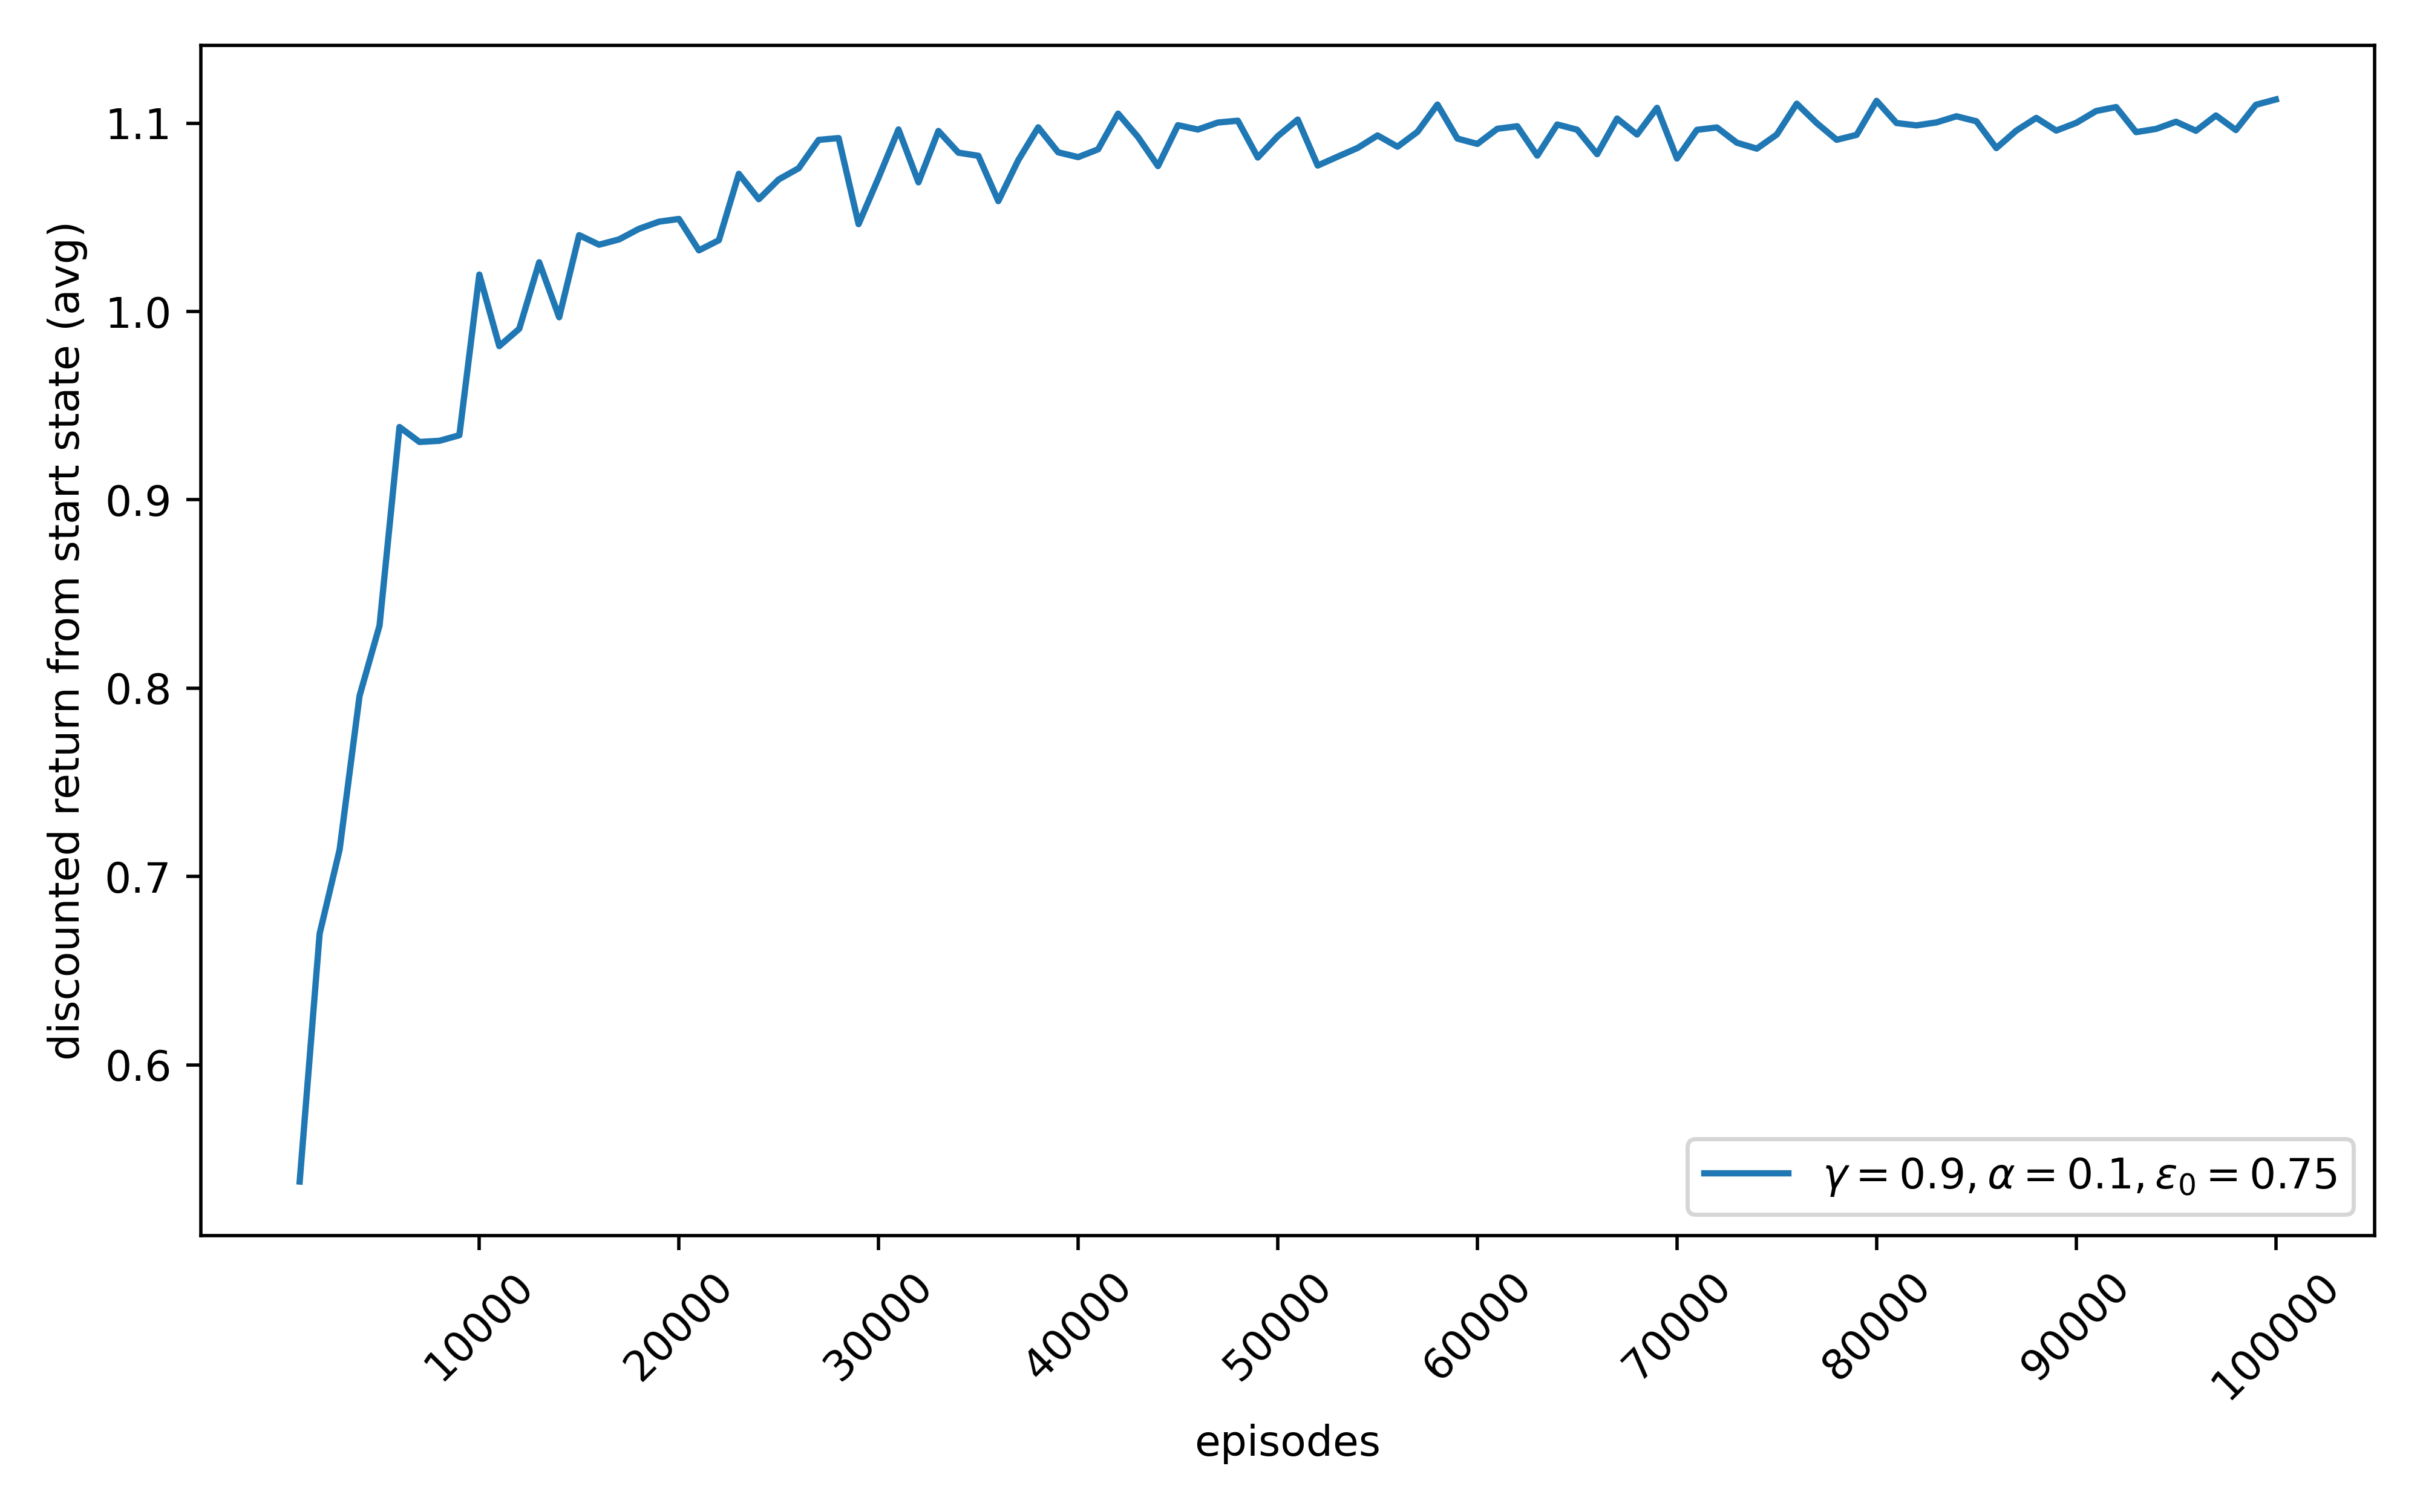
\includegraphics[width=\linewidth]{plots/part1-a-rewards.png}
        \caption{Discounted Return}
        
    \end{minipage}
    \hfill
    \begin{minipage}{0.49\linewidth}
        \centering
        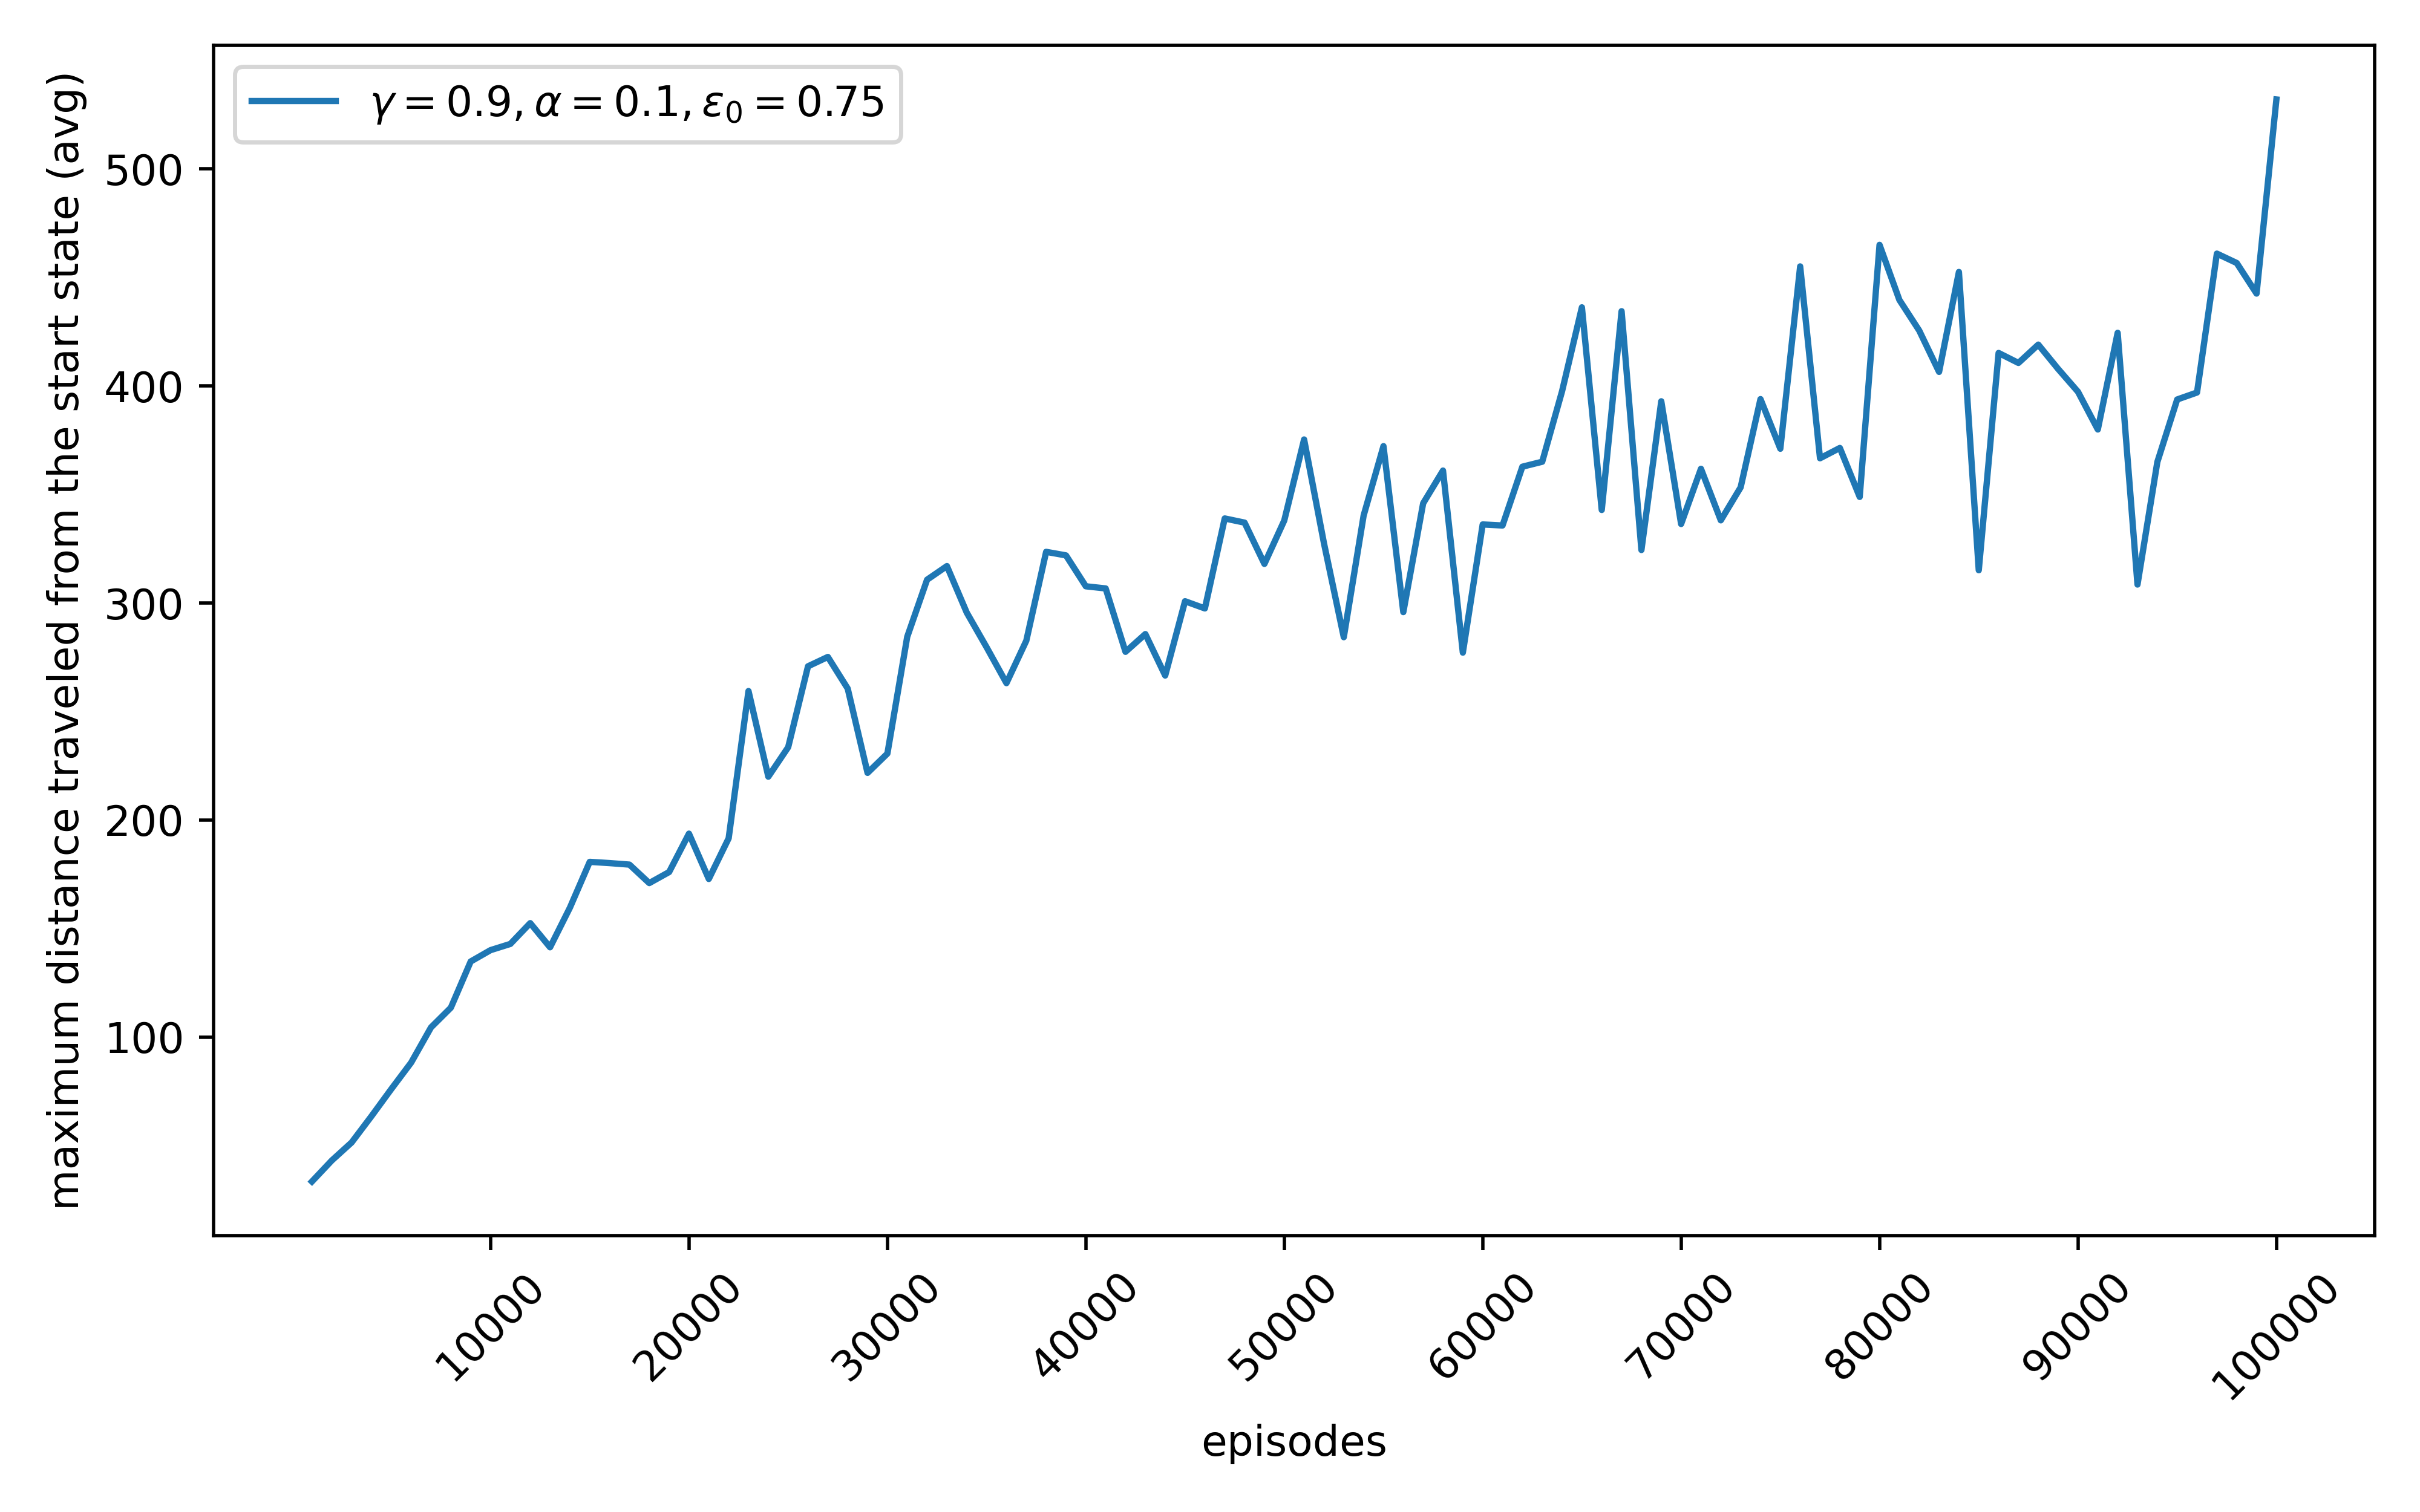
\includegraphics[width=\linewidth]{plots/part1-a-distances.png}
        \caption{Distance Traveled}
    \end{minipage}

    \vspace{1em}
    \begin{minipage}{\linewidth}
        \centering
        \begin{tabular}{lccc}
            \hline
            Episodes & Discounted Return & Average Distance \\
            \hline
            $50,000$ & $1.09$ & $338.00$ \\
            $98,000$ & $1.10$ & $456.64$ \\
            $99,000$ & $1.11$ & $442.55$ \\
            $100,000$ & $1.11$ & $531.98$ \\
            \hline
        \end{tabular}
        \caption{\texttt{Tabular} $\gamma = 0.9, \alpha = 0.1, \epsilon = 0.75$}
    \end{minipage}
     \label{fig:part1-a}
\end{figure}
\subsection{Lane Visualization}

\begin{enumerate}
\item See \autoref{fig:part1-a-lane-visualization}. \texttt{Black} to \texttt{white} represents increasing Q-value. Note that colors in two different visualizations are not to the same scale.
\item The agent assigns highest value to the lane where it can avoid collision for the longest time.
\item The agent also seems to value a lane based on value if lane(s) adjacent to it. 
\end{enumerate}

\begin{figure}[H]
    \centering
    \begin{minipage}[t]{0.48\textwidth}
        \centering
        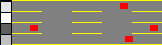
\includegraphics[width=\linewidth]{plots/part1-a-lane_visualization_00_step_0240.png}
    \end{minipage}
    \hfill
    \begin{minipage}[t]{0.48\textwidth}
        \centering
        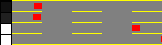
\includegraphics[width=\linewidth]{plots/part1-a-lane_visualization_00_step_0260.png}
    \end{minipage}
    
    \vspace{2mm}
    
    \begin{minipage}[t]{0.48\textwidth}
        \centering
        
\includegraphics[width=\linewidth]{plots/part1-a-lane_visualization_01_step_0340.png}
    \end{minipage}
    \hfill
    \begin{minipage}[t]{0.48\textwidth}
        \centering
        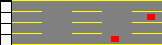
\includegraphics[width=\linewidth]{plots/part1-a-lane_visualization_01_step_0600.png}
    \end{minipage}
    \caption{Lane visualization for Tabular Q-agent}
    \label{fig:part1-a-lane-visualization}
\end{figure}

\subsection{Speed Visualization}
\begin{enumerate}
\item Note that \texttt{speed = 4} is always black due to the environment.
\item See \autoref{fig:part1-a-speed-visualization}. The agent prefers higher speed when the obstacle is farther away.
\end{enumerate}

\begin{figure}[H]
    \centering
    \begin{minipage}{0.48\textwidth}
        \centering
        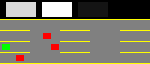
\includegraphics[width=\linewidth]{plots/part1-a-speed_visualization_00_step_0120.png}
    \end{minipage}
    \hfill
    \begin{minipage}{0.48\textwidth}
        \centering
        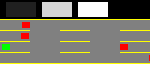
\includegraphics[width=\linewidth]{plots/part1-a-speed_visualization_00_step_0260.png}
    \end{minipage}
    \caption{Speed visualization for Tabular Q-agent}
    \label{fig:part1-a-speed-visualization}
\end{figure}





\subsection{Varying $\gamma$}
\begin{figure}[H]
    \centering
    \begin{minipage}{0.49\linewidth}
        \centering
        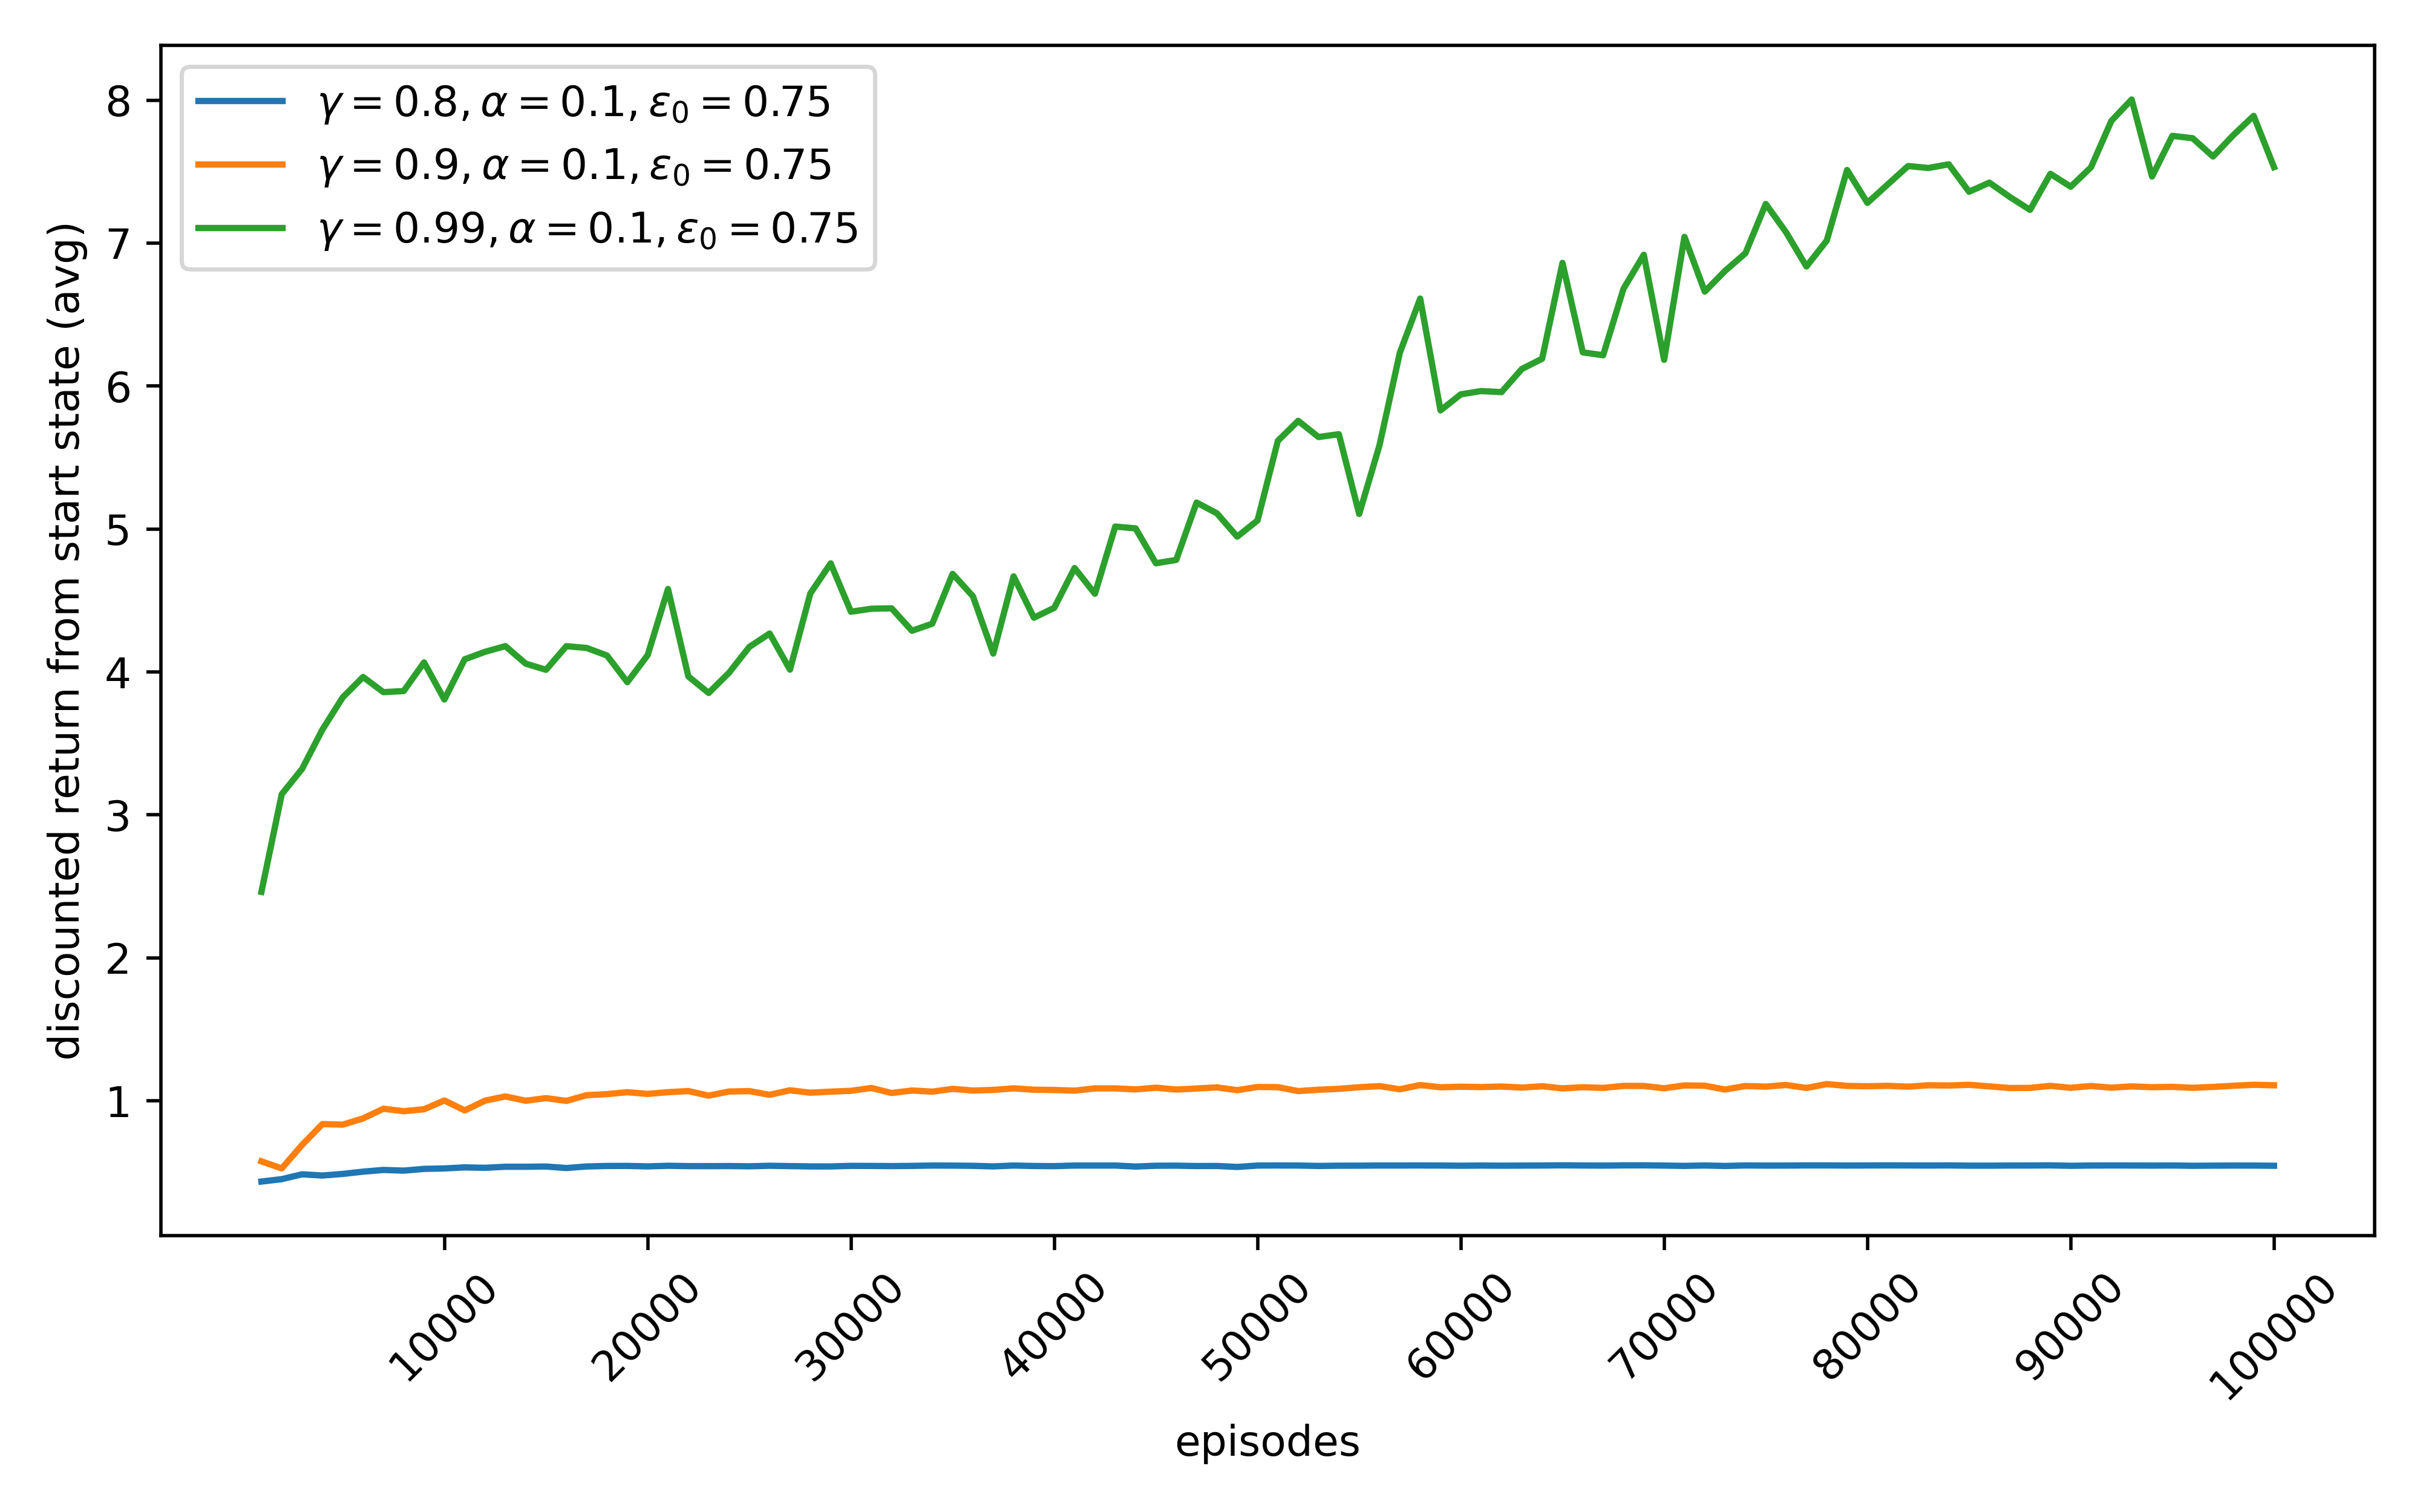
\includegraphics[width=\linewidth]{plots/part1-b-rewards.png}
        \caption{Discounted Return}
    \end{minipage}
    \hfill
    \begin{minipage}{0.49\linewidth}
        \centering
        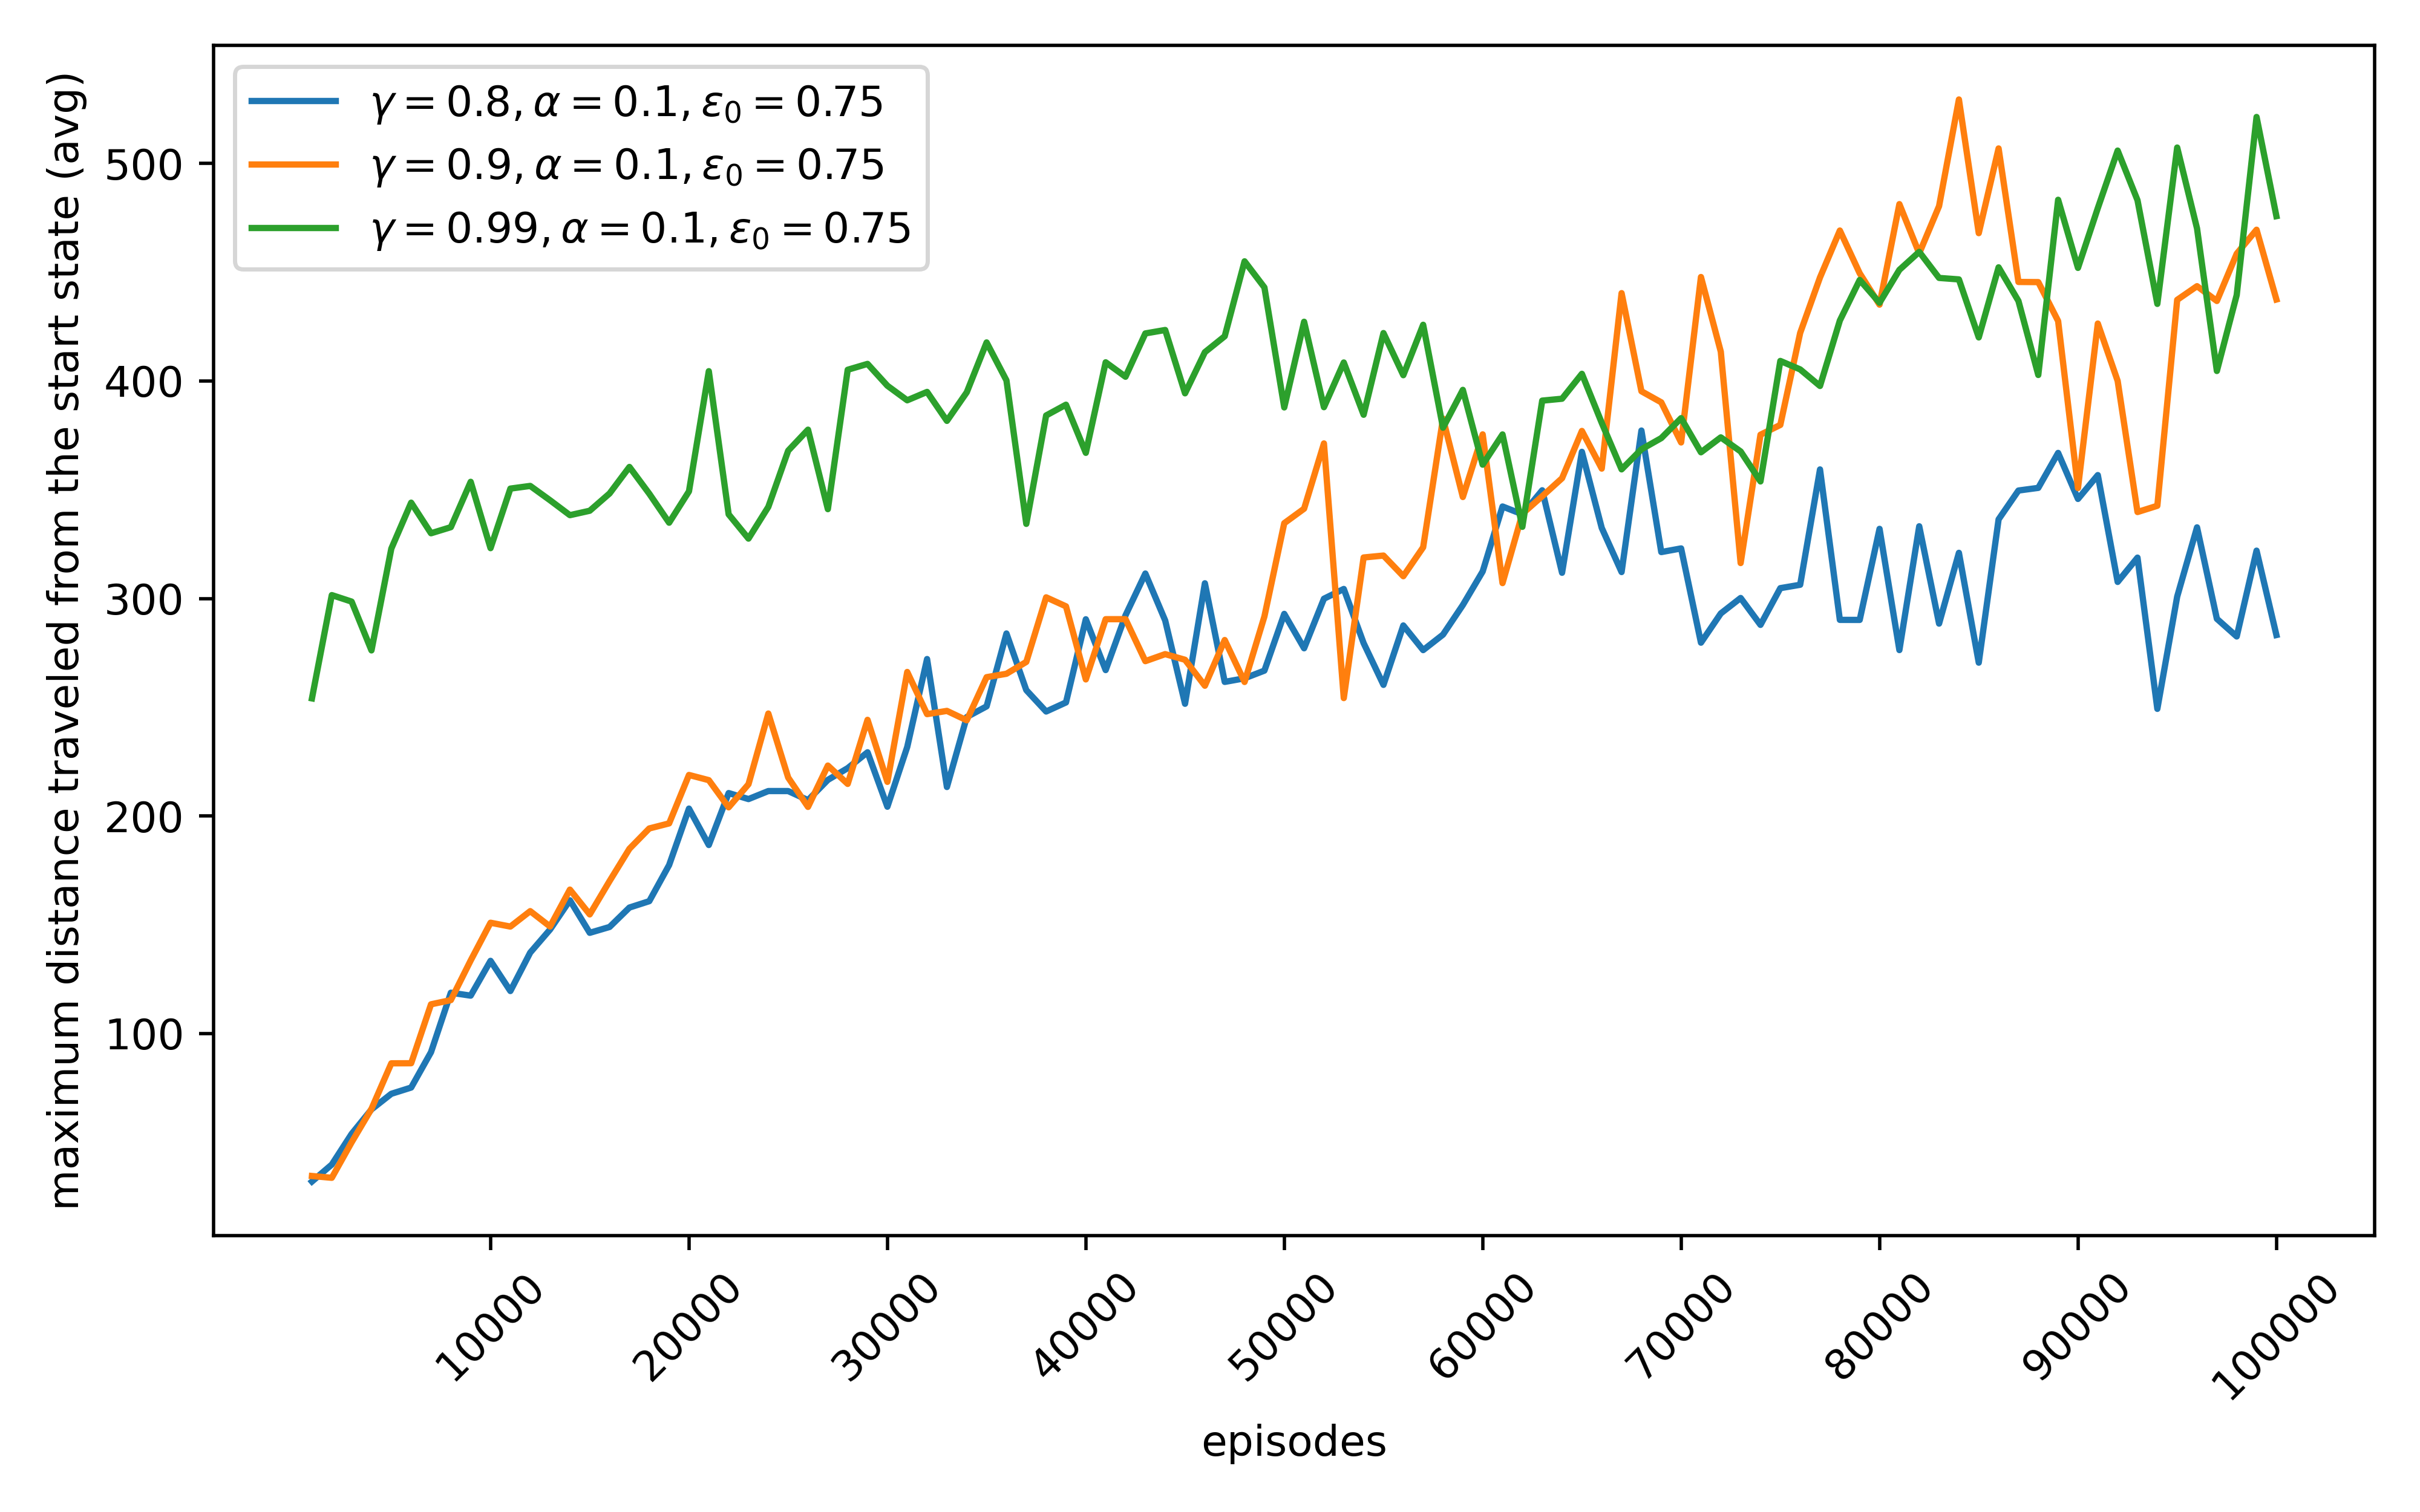
\includegraphics[width=\linewidth]{plots/part1-b-distances.png}
        \caption{Distance Traveled}
    \end{minipage}

    \vspace{1em}
    \begin{minipage}{\linewidth}
        \centering
        \begin{tabular}{lccc}
            \hline
            $\gamma$ & Discounted Return & Average Distance \\
            \hline
            $0.80$ & $0.55$ & $283.21$ \\
            $0.90$ & $1.11$ & $437.49$ \\
            $0.99$ & $7.53$ & $475.81$ \\
            \hline
        \end{tabular}
        \caption{\texttt{Tabular} $100,000$ iterations, $\alpha = 0.1, \epsilon = 0.75$}
    \end{minipage}
     \label{fig:part1-b}
\end{figure}
Increase in the discount factor tends to lead to a significant increase in the discounted returns, (as upper bound on discounted returns is $\frac{0.12}{1 - \gamma}$)  and a general increase in the average distance traveled. The reason is discussed in \nameref{sec:reward-goal}.




\subsection{Varying $\alpha$}

\begin{figure}[H]
    \centering
    \begin{minipage}{0.49\linewidth}
        \centering
        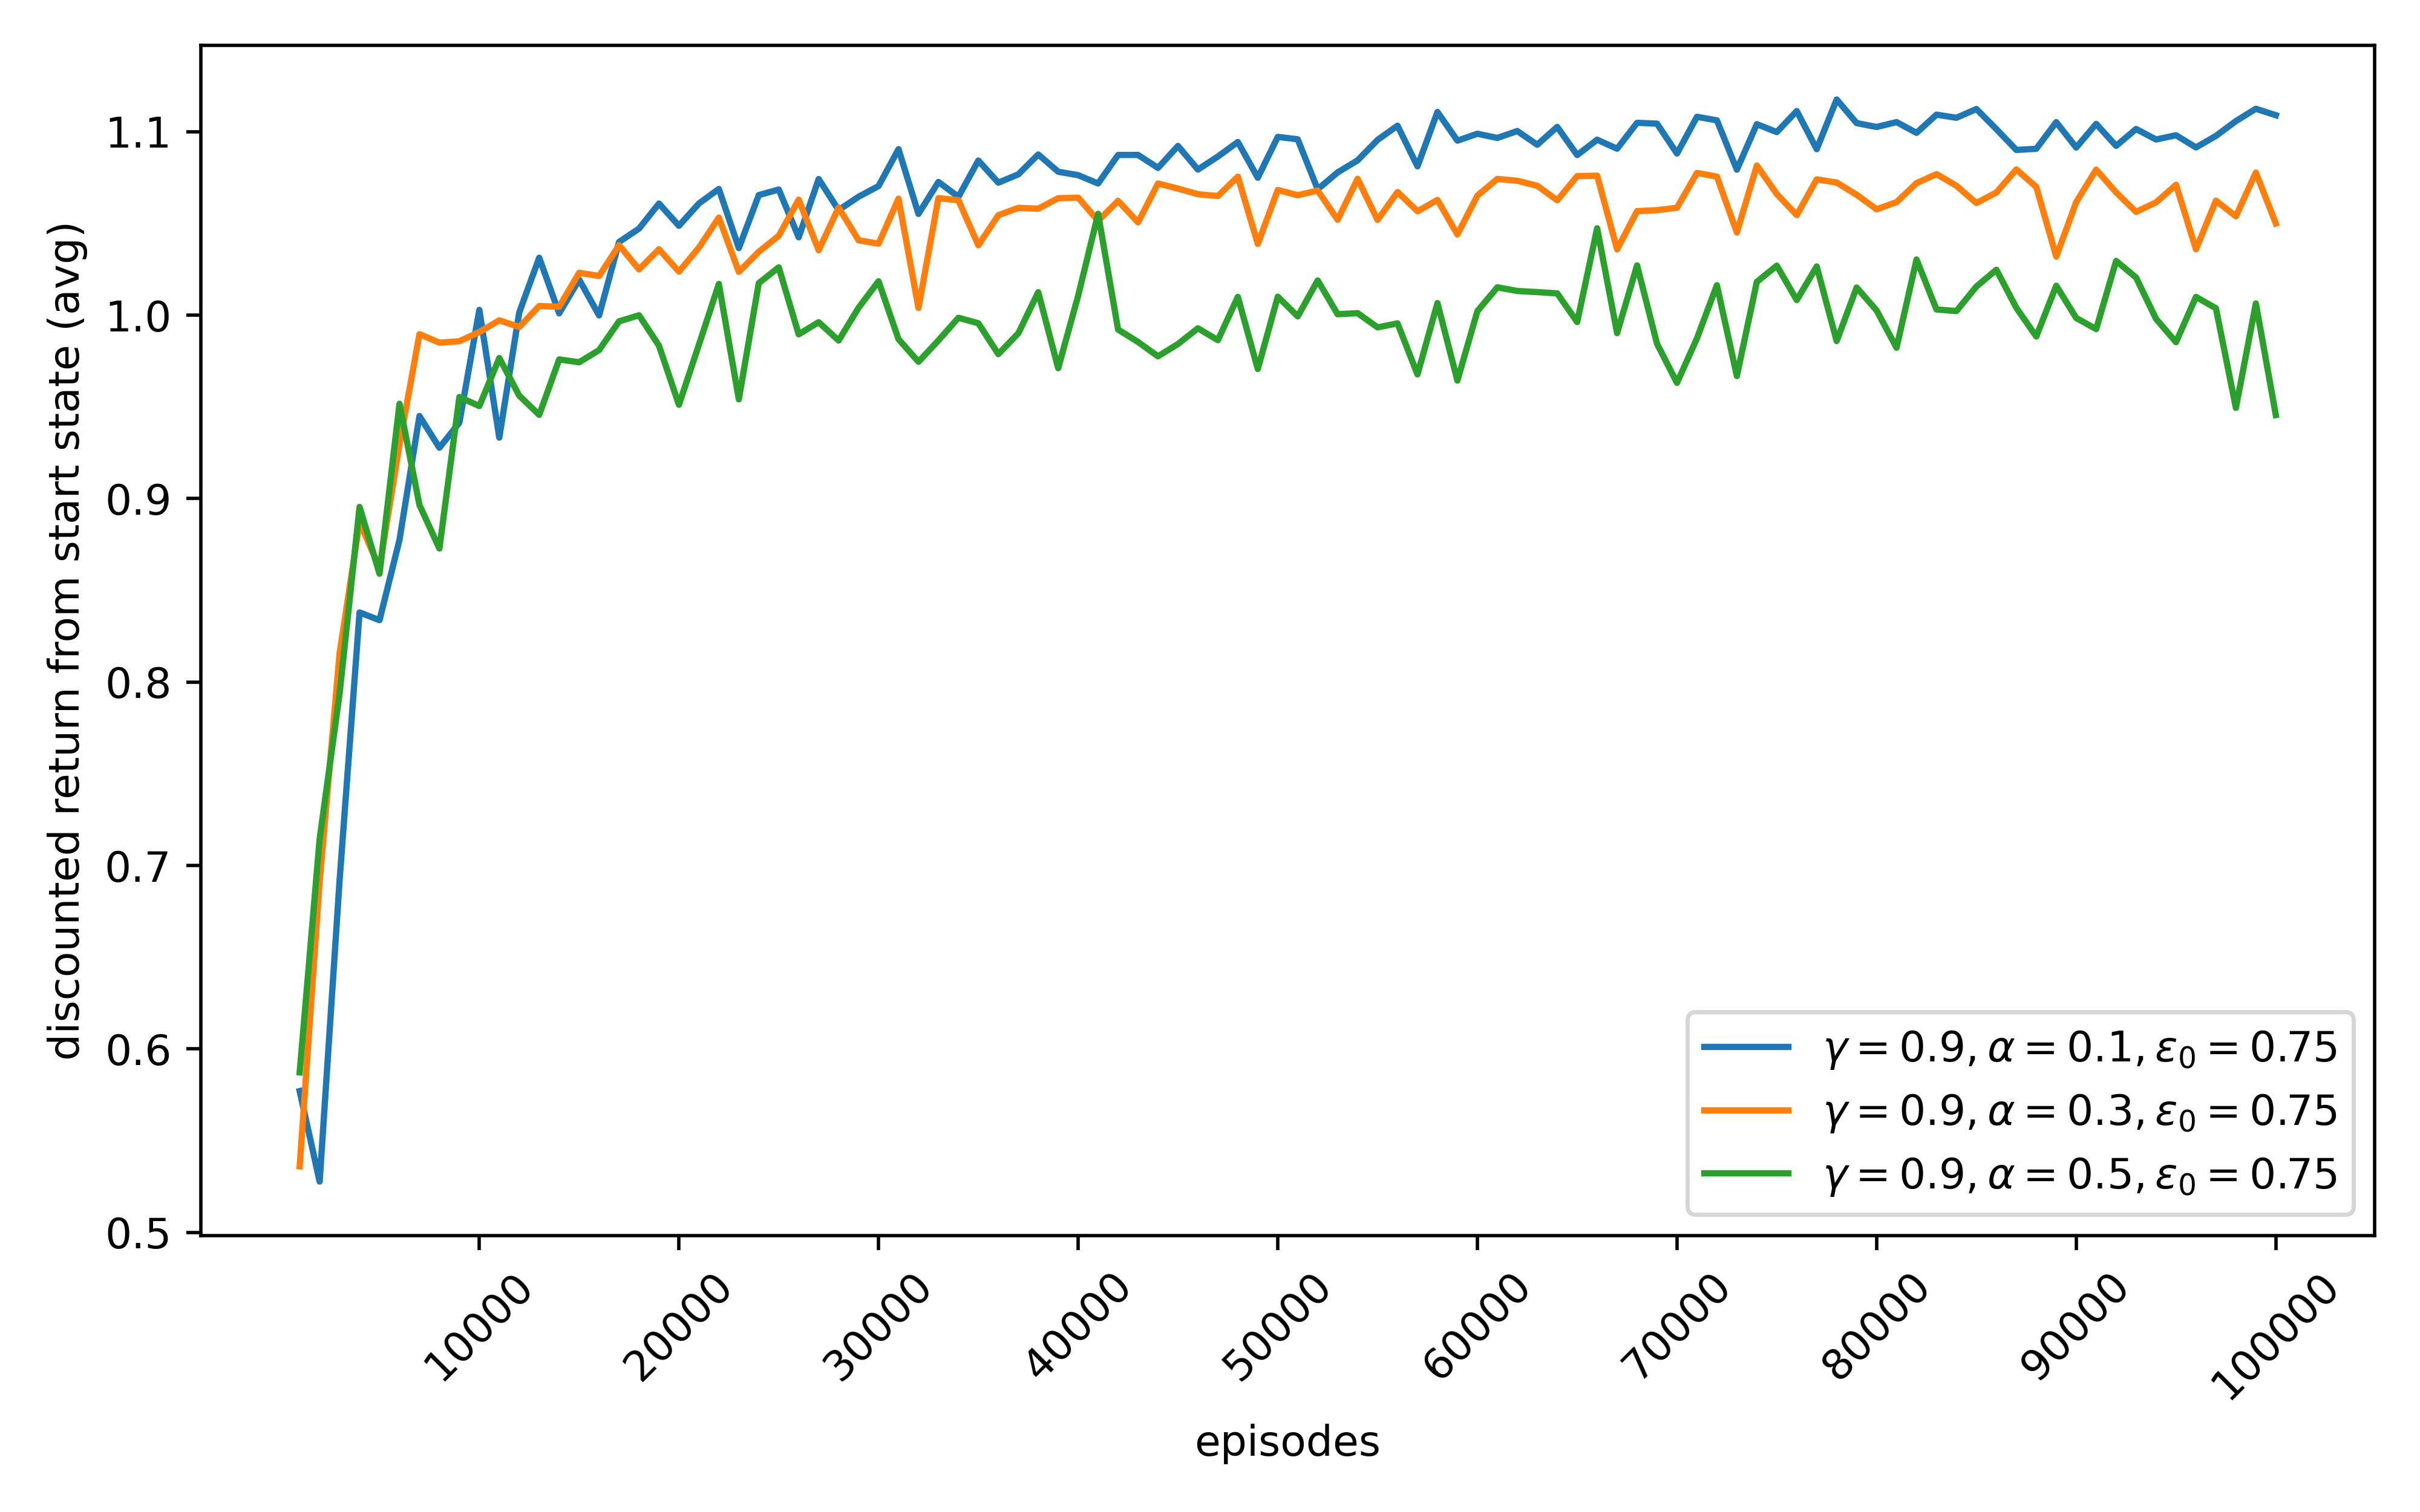
\includegraphics[width=\linewidth]{plots/part1-c-rewards.png}
        \caption{Discounted Return}
    \end{minipage}
    \hfill
    \begin{minipage}{0.49\linewidth}
        \centering
        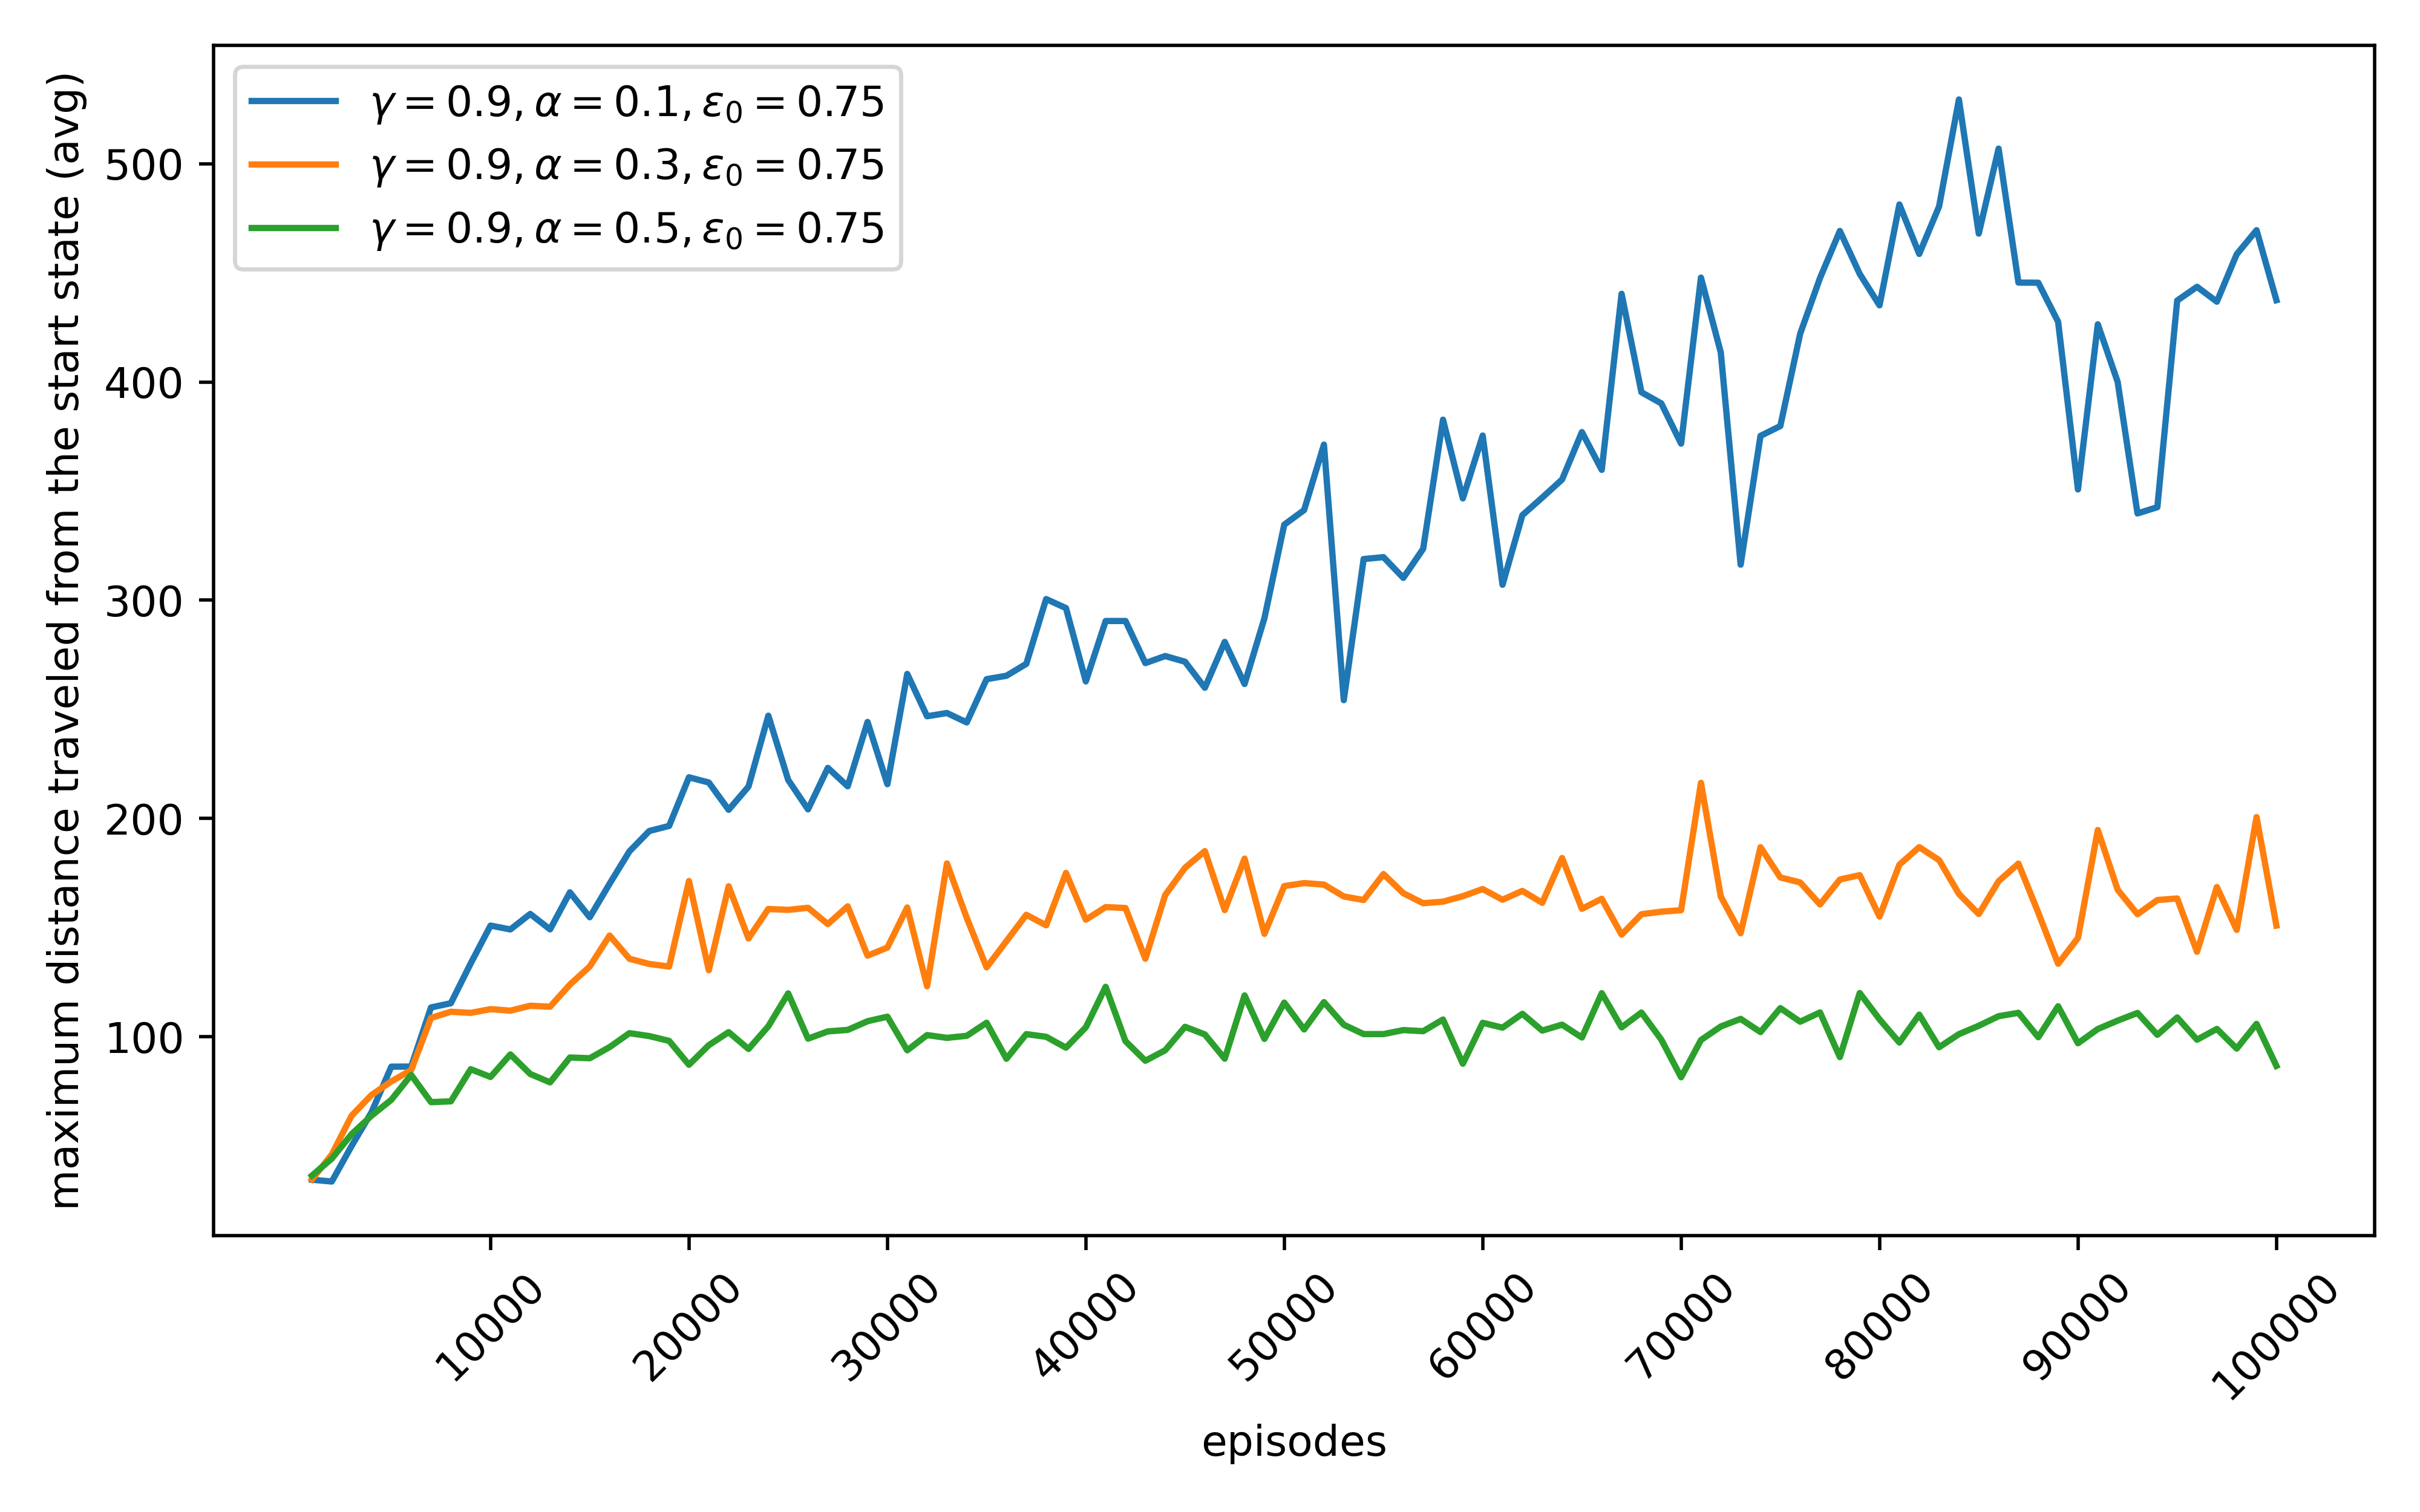
\includegraphics[width=\linewidth]{plots/part1-c-distances.png}
        \caption{Distance Traveled}
    \end{minipage}

    \vspace{1em}
    \begin{minipage}{\linewidth}
    \centering
    \begin{tabular}{lccc}
        \hline
     $\alpha$ & Discounted Return & Average Distance \\
        \hline
    $0.1$ & $1.11$ & $437.49$ \\
    $0.3$ & $1.05$ & $150.90$ \\
    $0.5$ & $0.95$ & $86.61$ \\
        \hline
    \end{tabular}
    \caption{\texttt{Tabular} $100,000$ iterations, $\gamma = 0.9, \epsilon = 0.75$} 
    \end{minipage}
     \label{fig:part1-c}
\end{figure}
In \texttt{Tabular} training, an update is made after every action. The batch size is $1$. Higher $\alpha$ means bigger updates leading to unstable training, and agent being biased towards later updates. Very briefly, during the initial few thousand episodes, higher $\alpha$ does better. Later, "forgetting" starts.


\subsection{Scheduling $\epsilon$}
\begin{figure}[H]
    \centering
    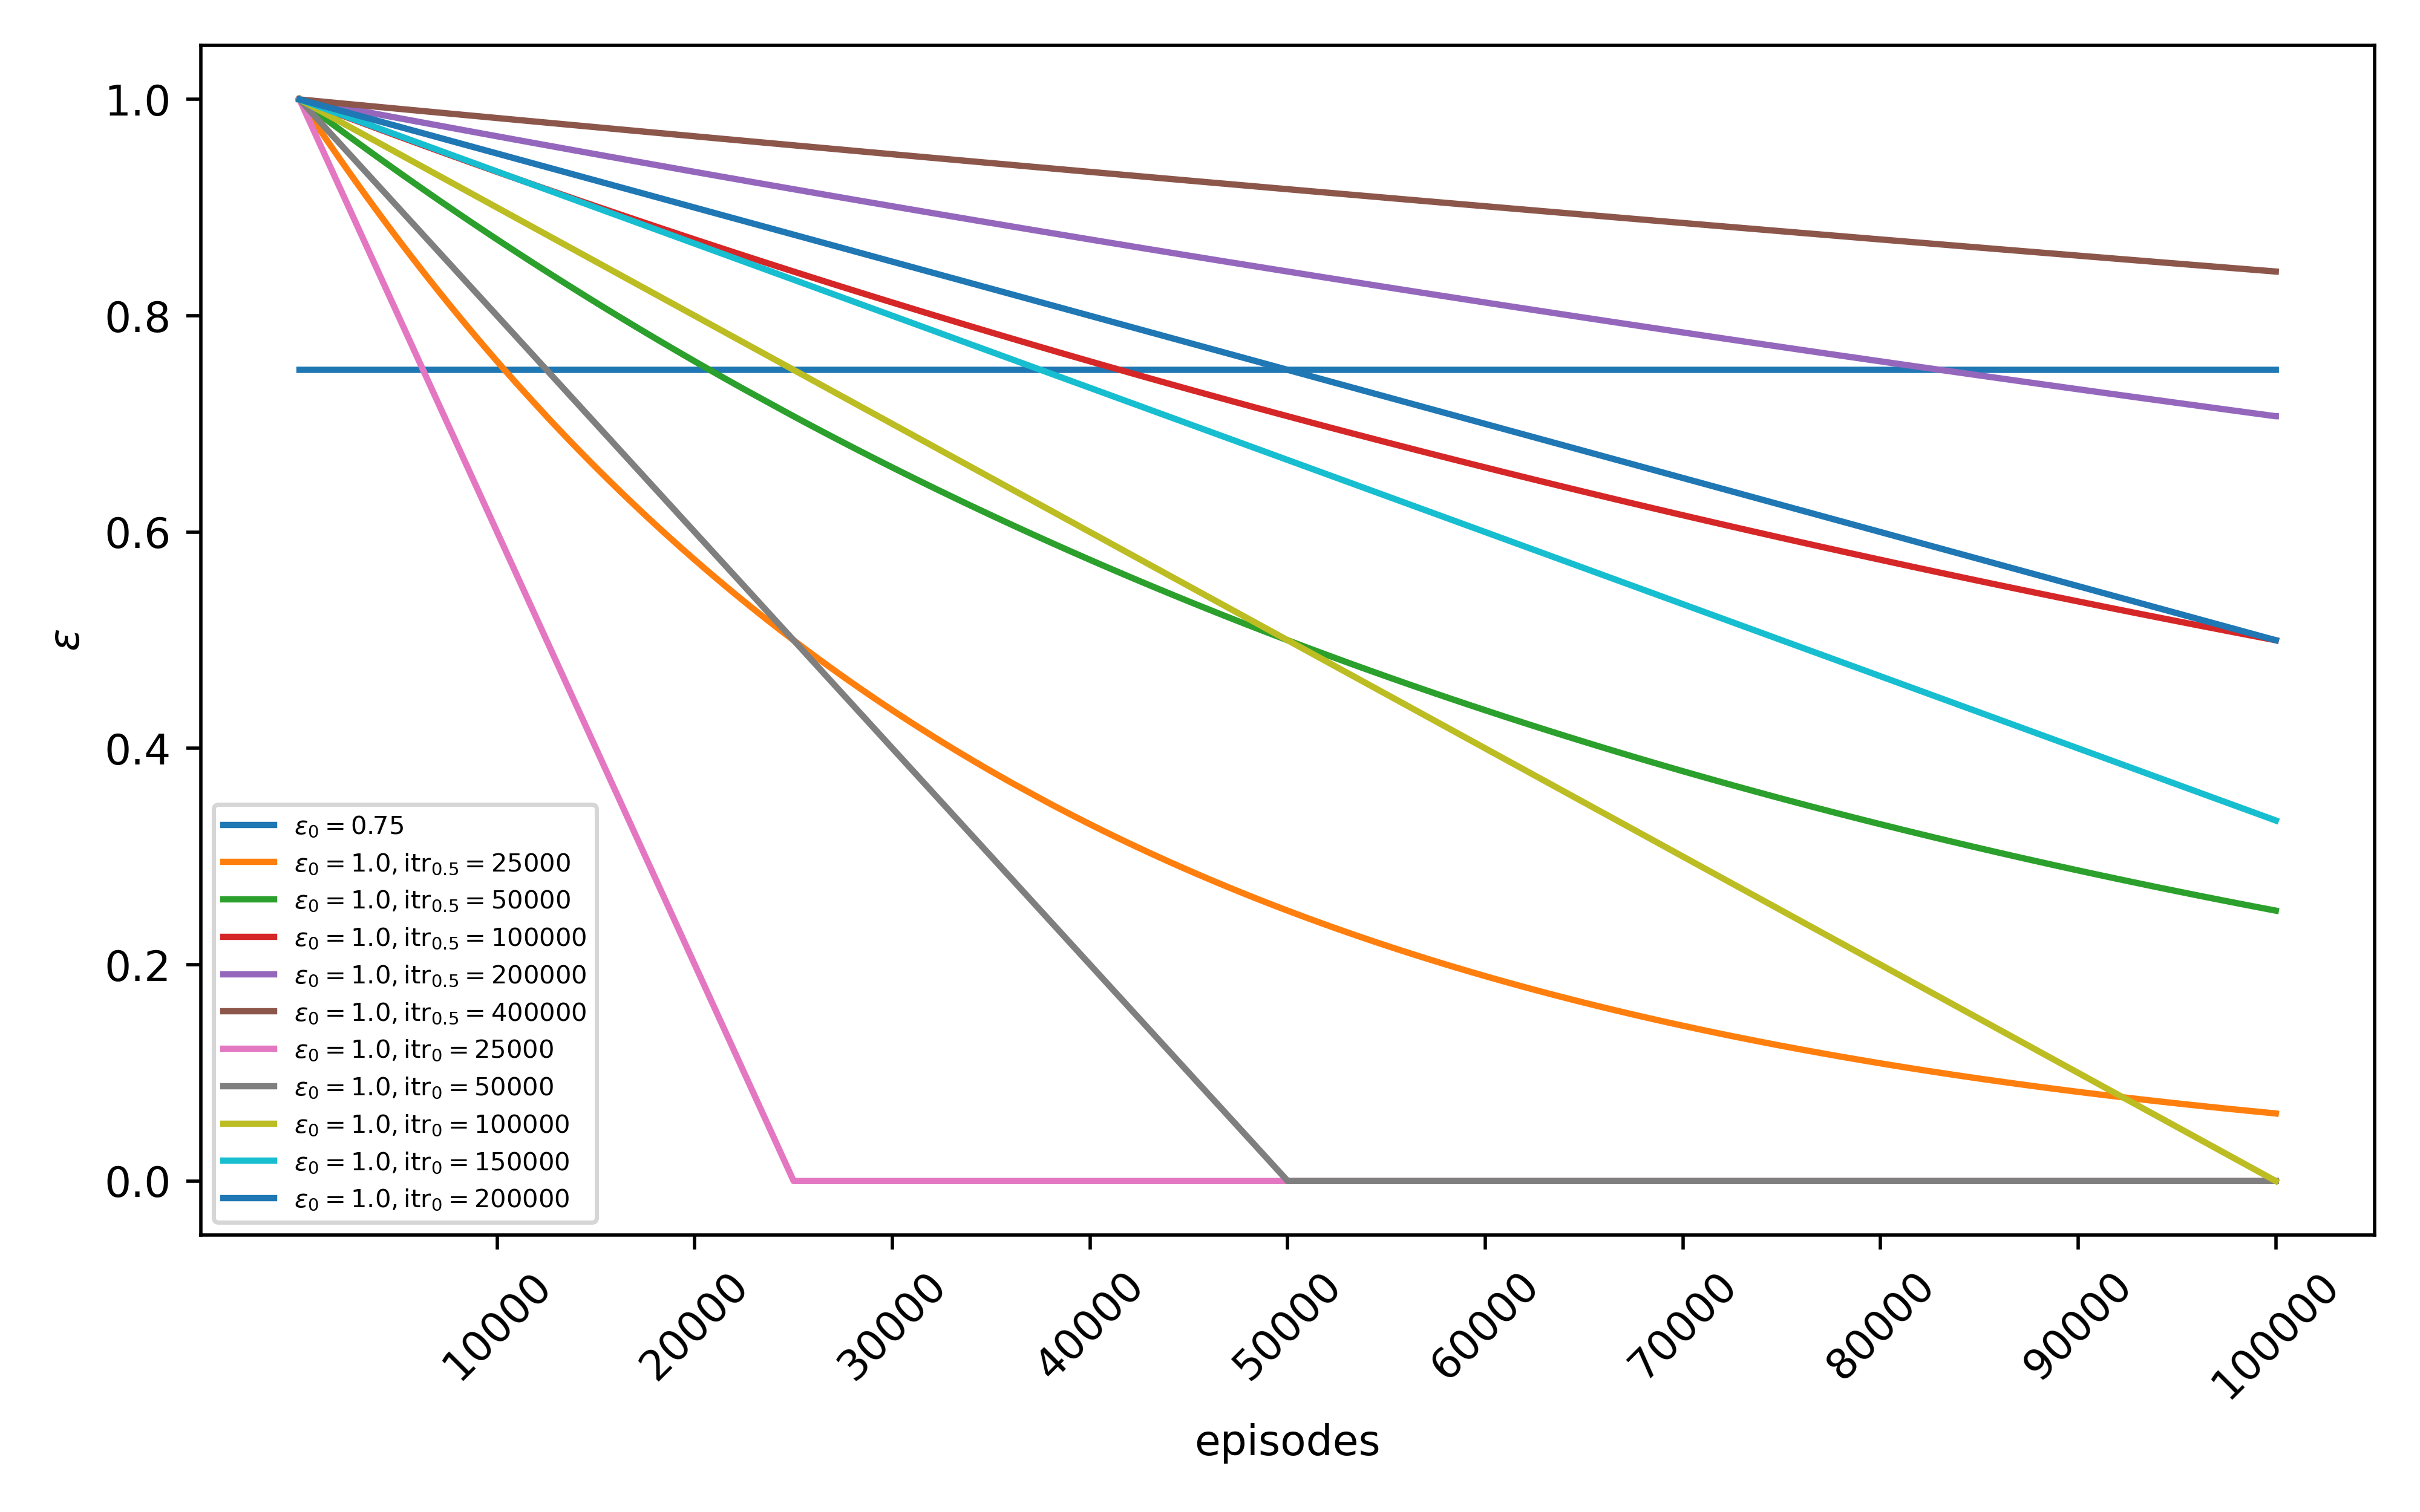
\includegraphics[width=0.5\linewidth]{plots/part1-d-epsilons.png}
    \caption{$\epsilon$ while training}
    \label{fig:part1-d-epsilons}
\end{figure}
\begin{figure}[H]
    \centering
    % First Row - Plots
    \begin{minipage}{0.32\linewidth}
        \centering
        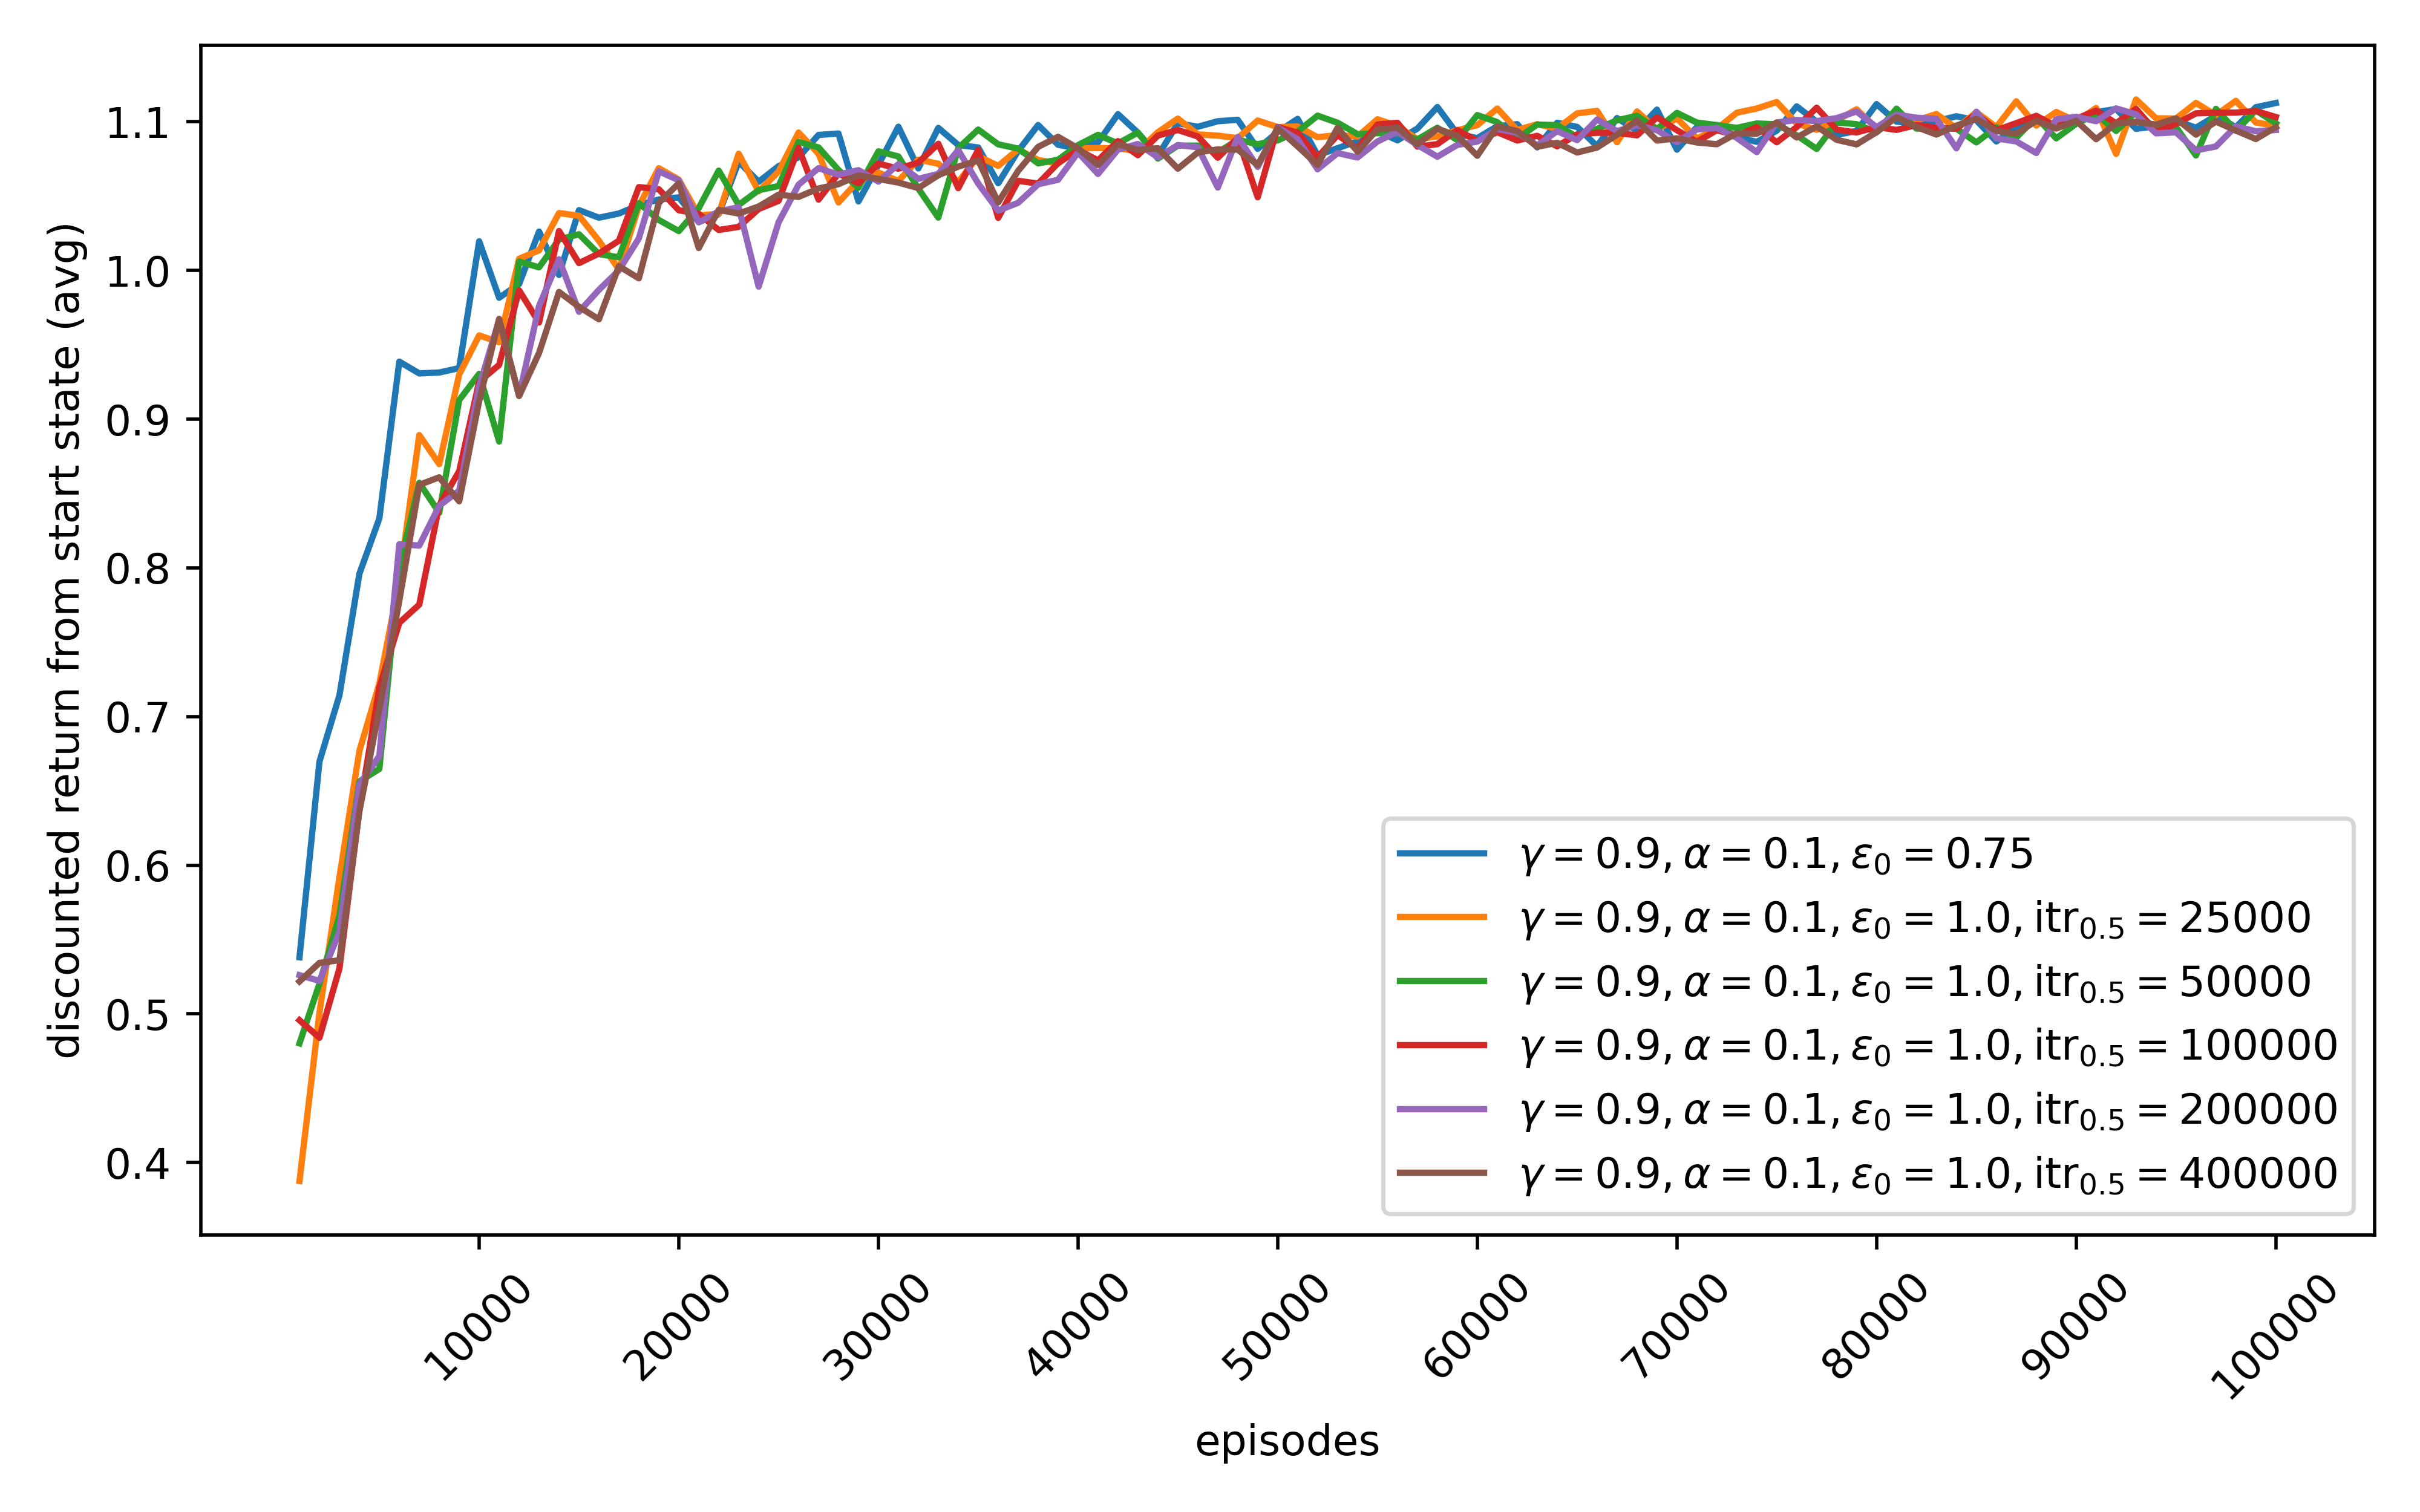
\includegraphics[width=\linewidth]{plots/part1-d.exponential-rewards.png}
        \caption{Discounted Return}
    \end{minipage}
    \hfill
    \begin{minipage}{0.32\linewidth}
        \centering
        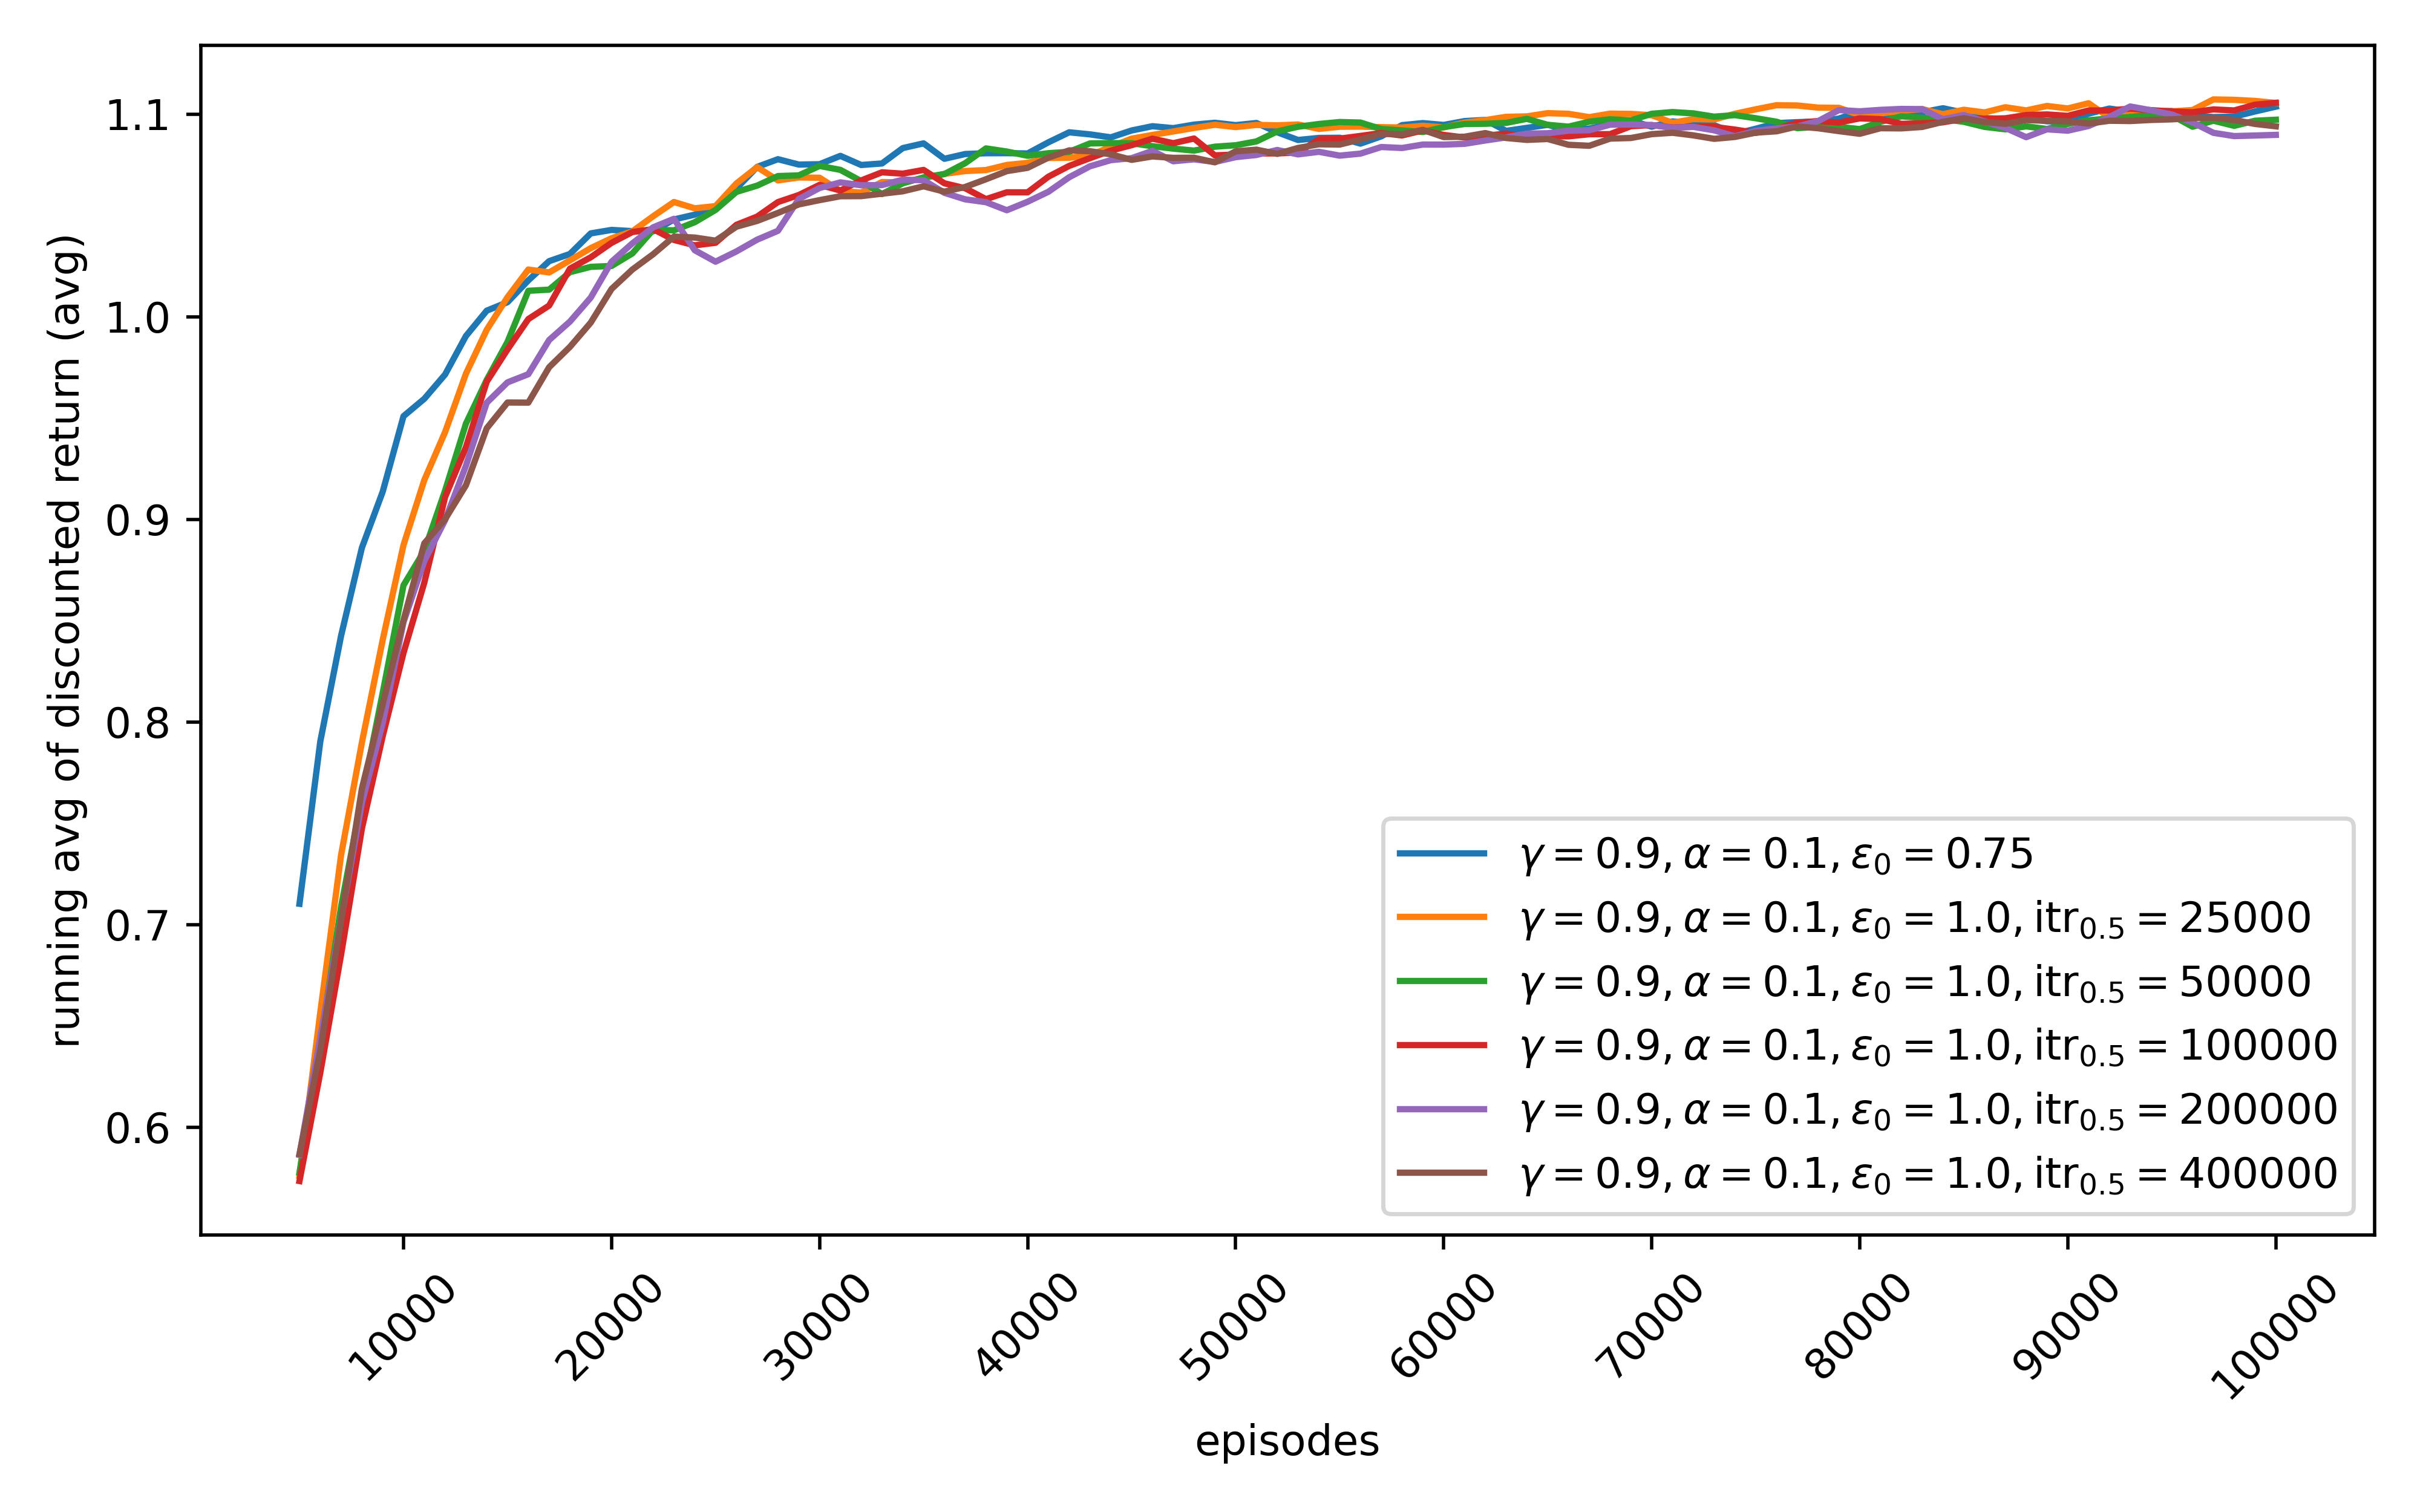
\includegraphics[width=\linewidth]{plots/part1-d.exponential-running_returns.png}
        \caption{Running Average of Discounted Return}
    \end{minipage}
    \hfill
    \begin{minipage}{0.32\linewidth}
        \centering
        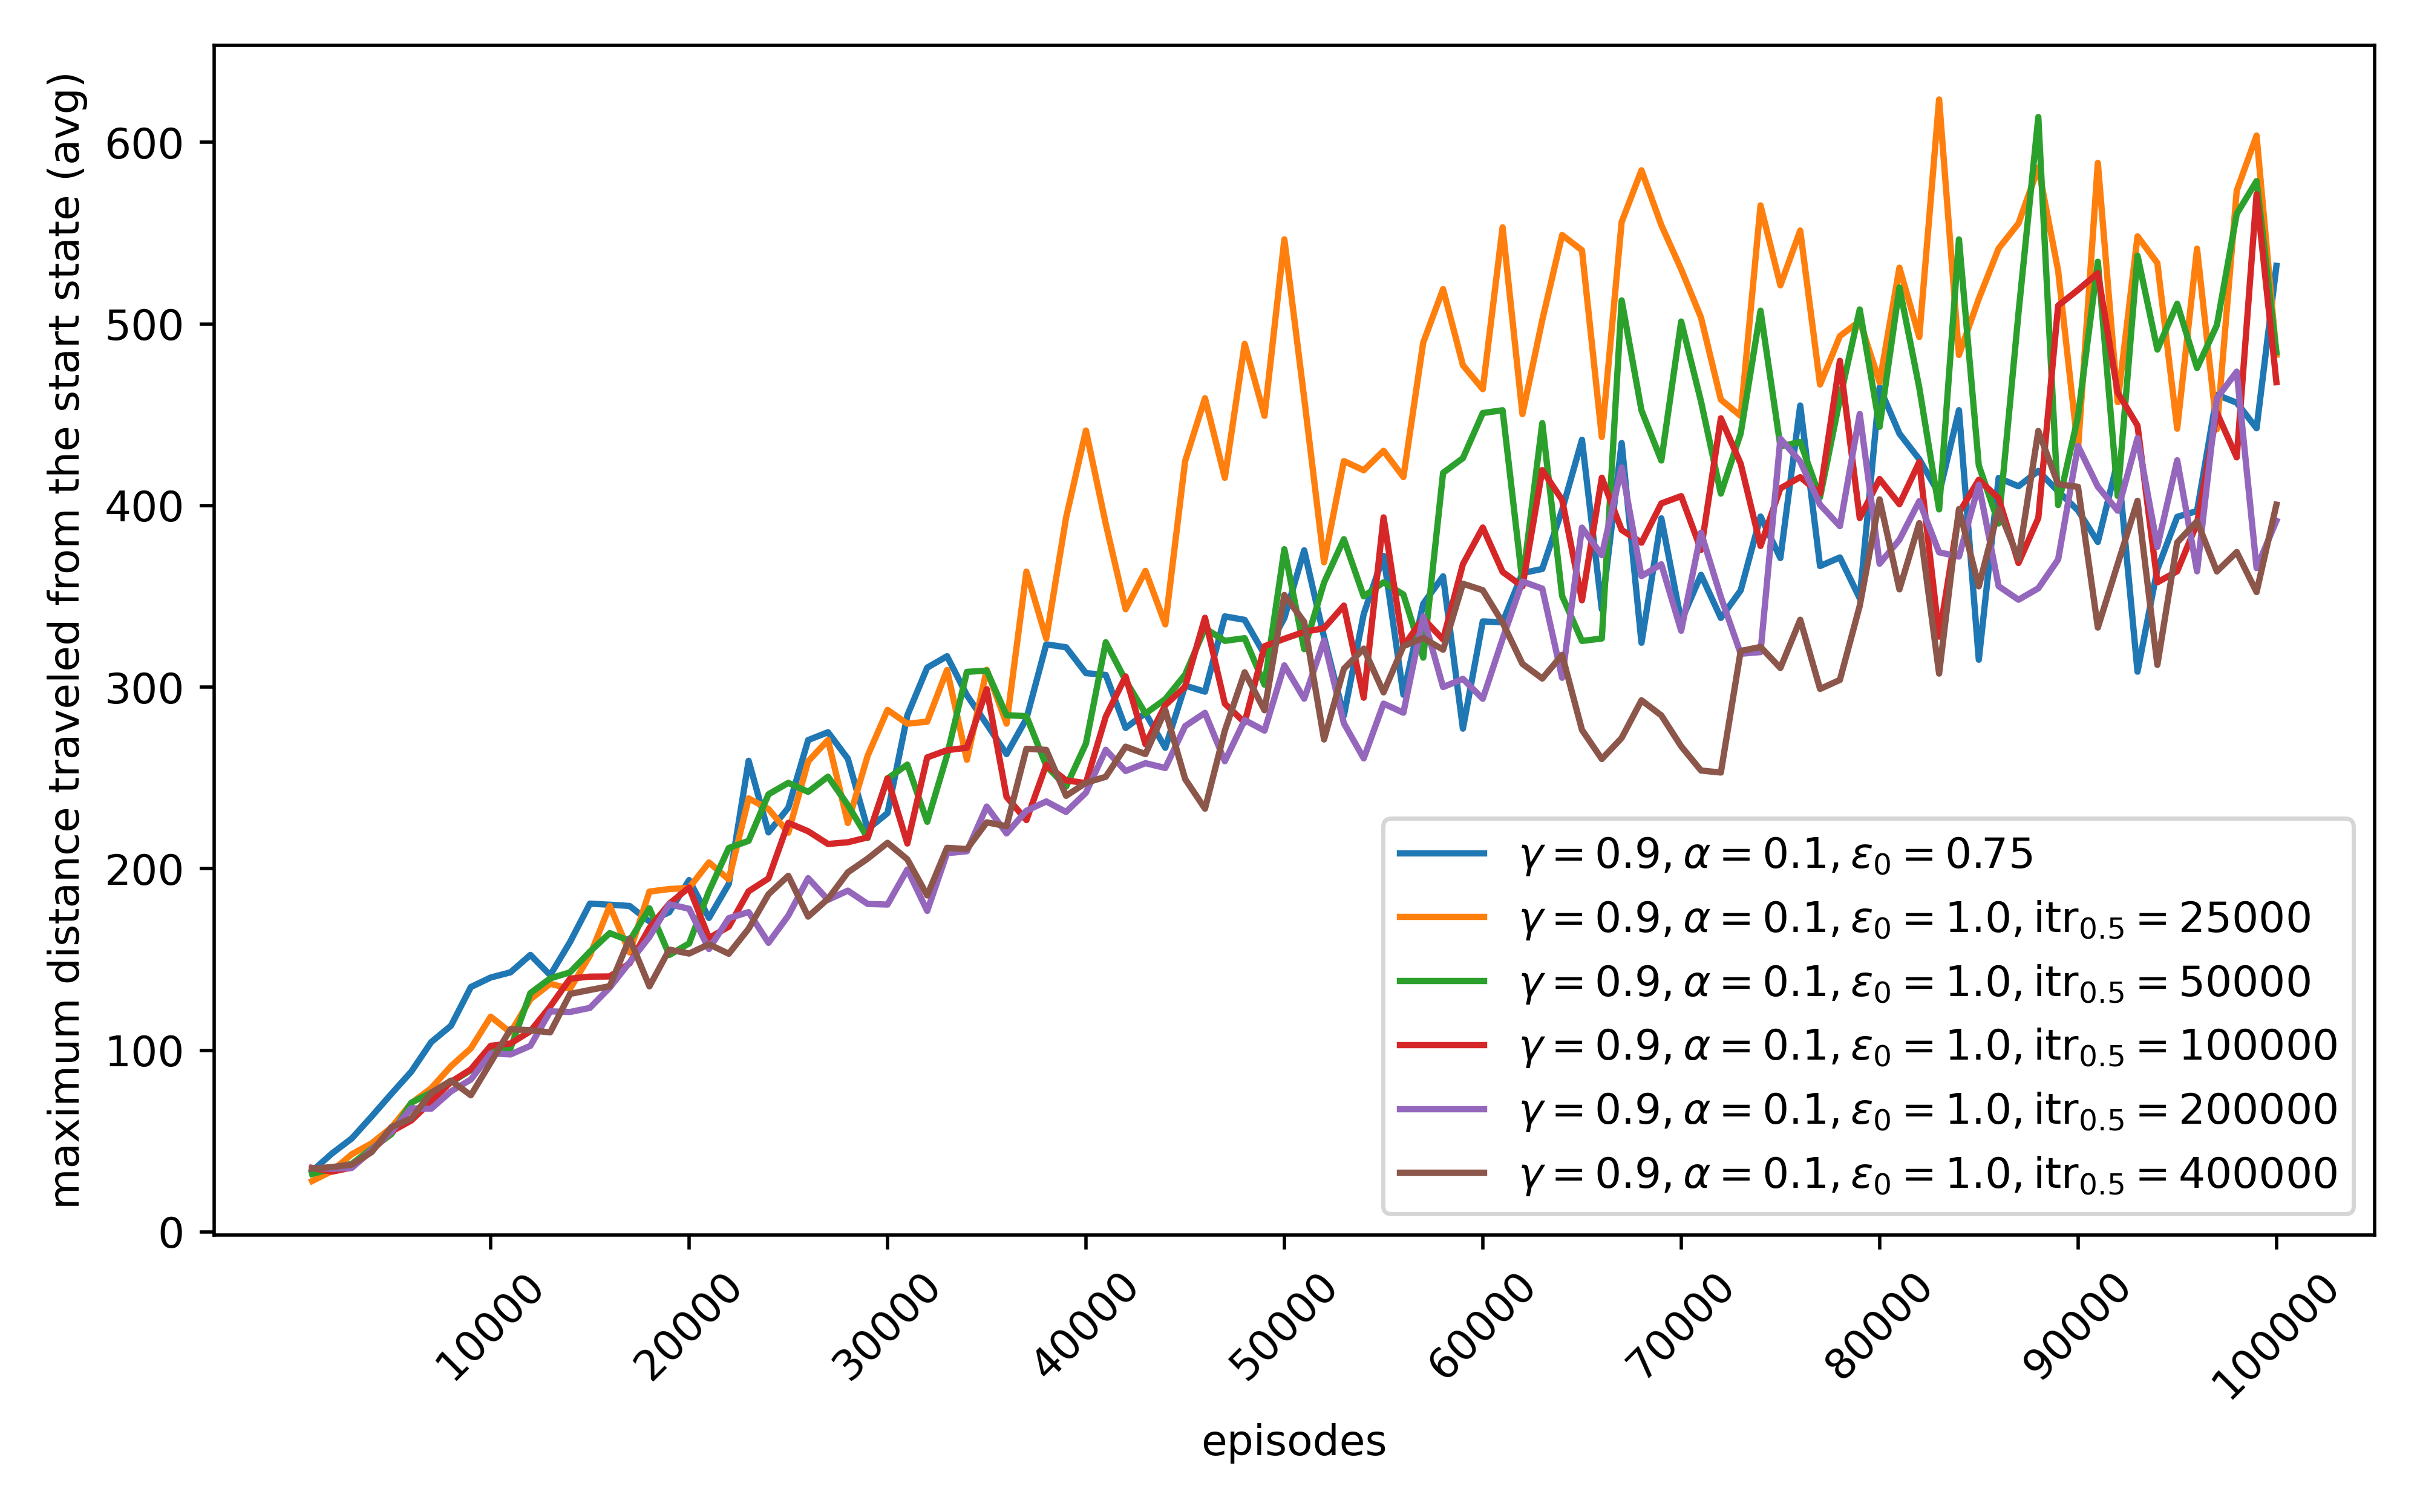
\includegraphics[width=\linewidth]{plots/part1-d.exponential-distances.png}
        \caption{Distance Traveled}
    \end{minipage}

    \vspace{0.5em}

    % Second Row - Plots
    \begin{minipage}{0.32\linewidth}
        \centering
        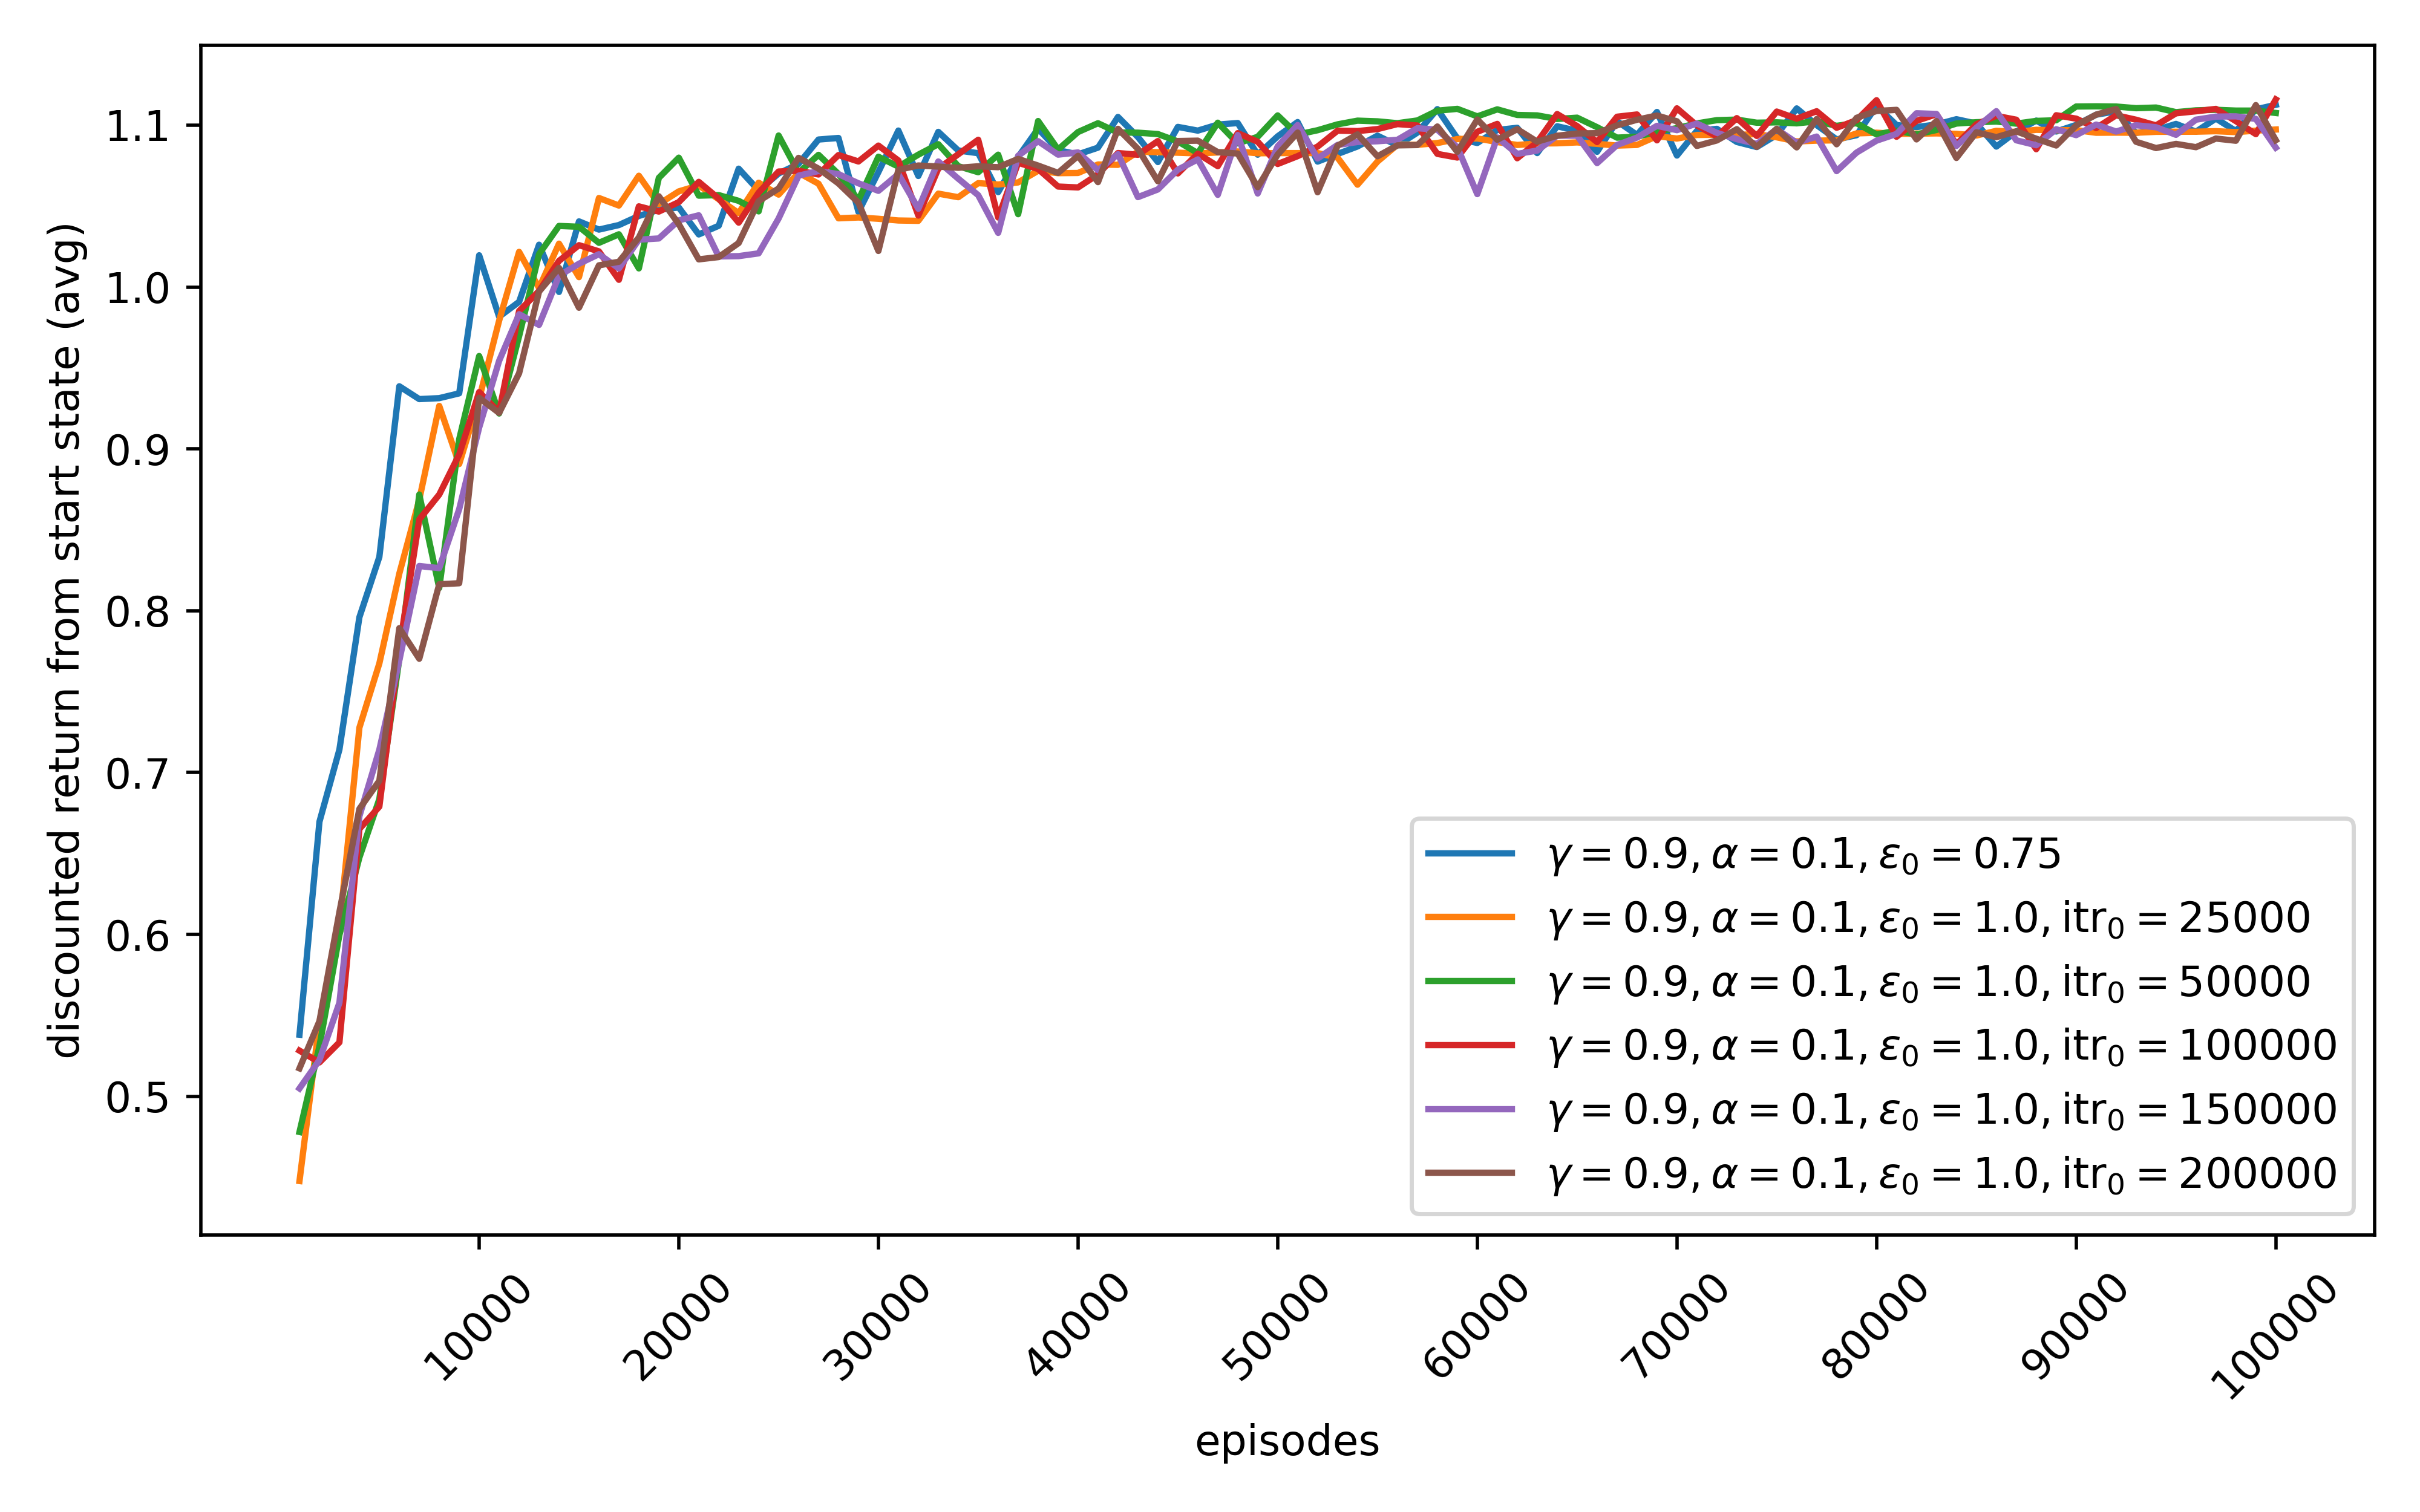
\includegraphics[width=\linewidth]{plots/part1-d.linear-rewards.png}
        \caption{Discounted Return}
    \end{minipage}
    \hfill
    \begin{minipage}{0.32\linewidth}
        \centering
        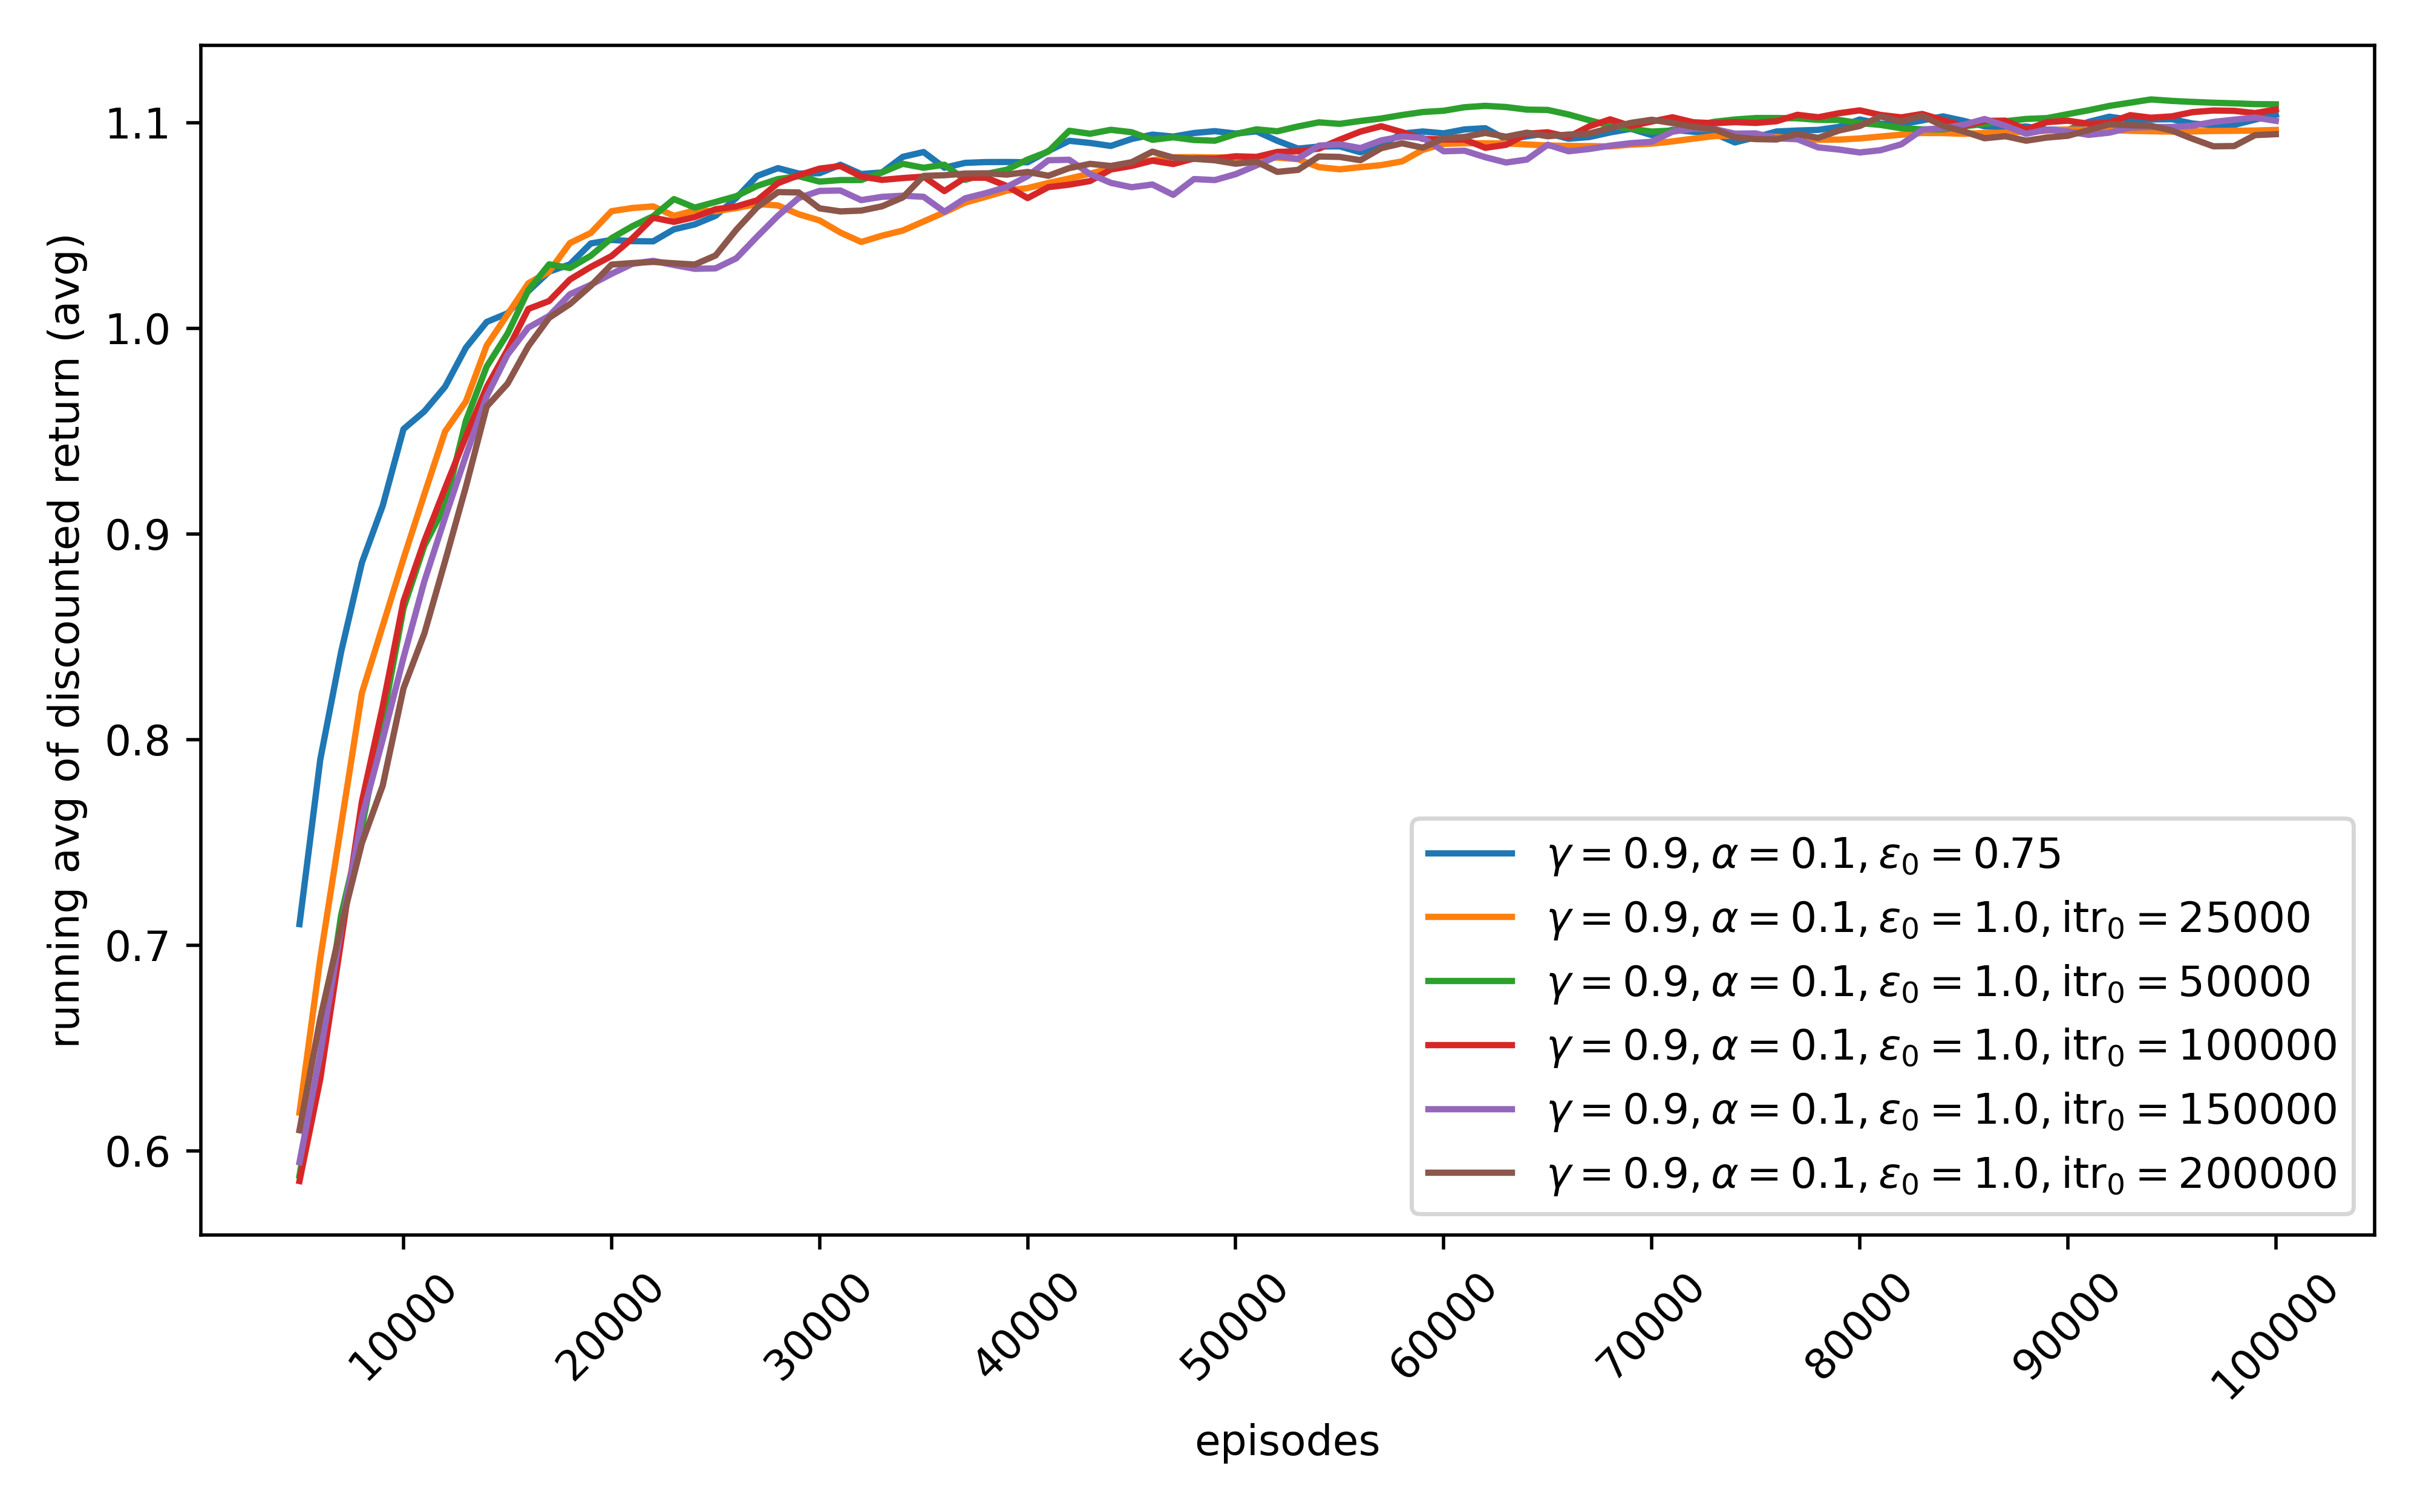
\includegraphics[width=\linewidth]{plots/part1-d.linear-running_returns.png}
        \caption{Running Average of Discounted Return}
    \end{minipage}
    \hfill
    \begin{minipage}{0.32\linewidth}
        \centering
        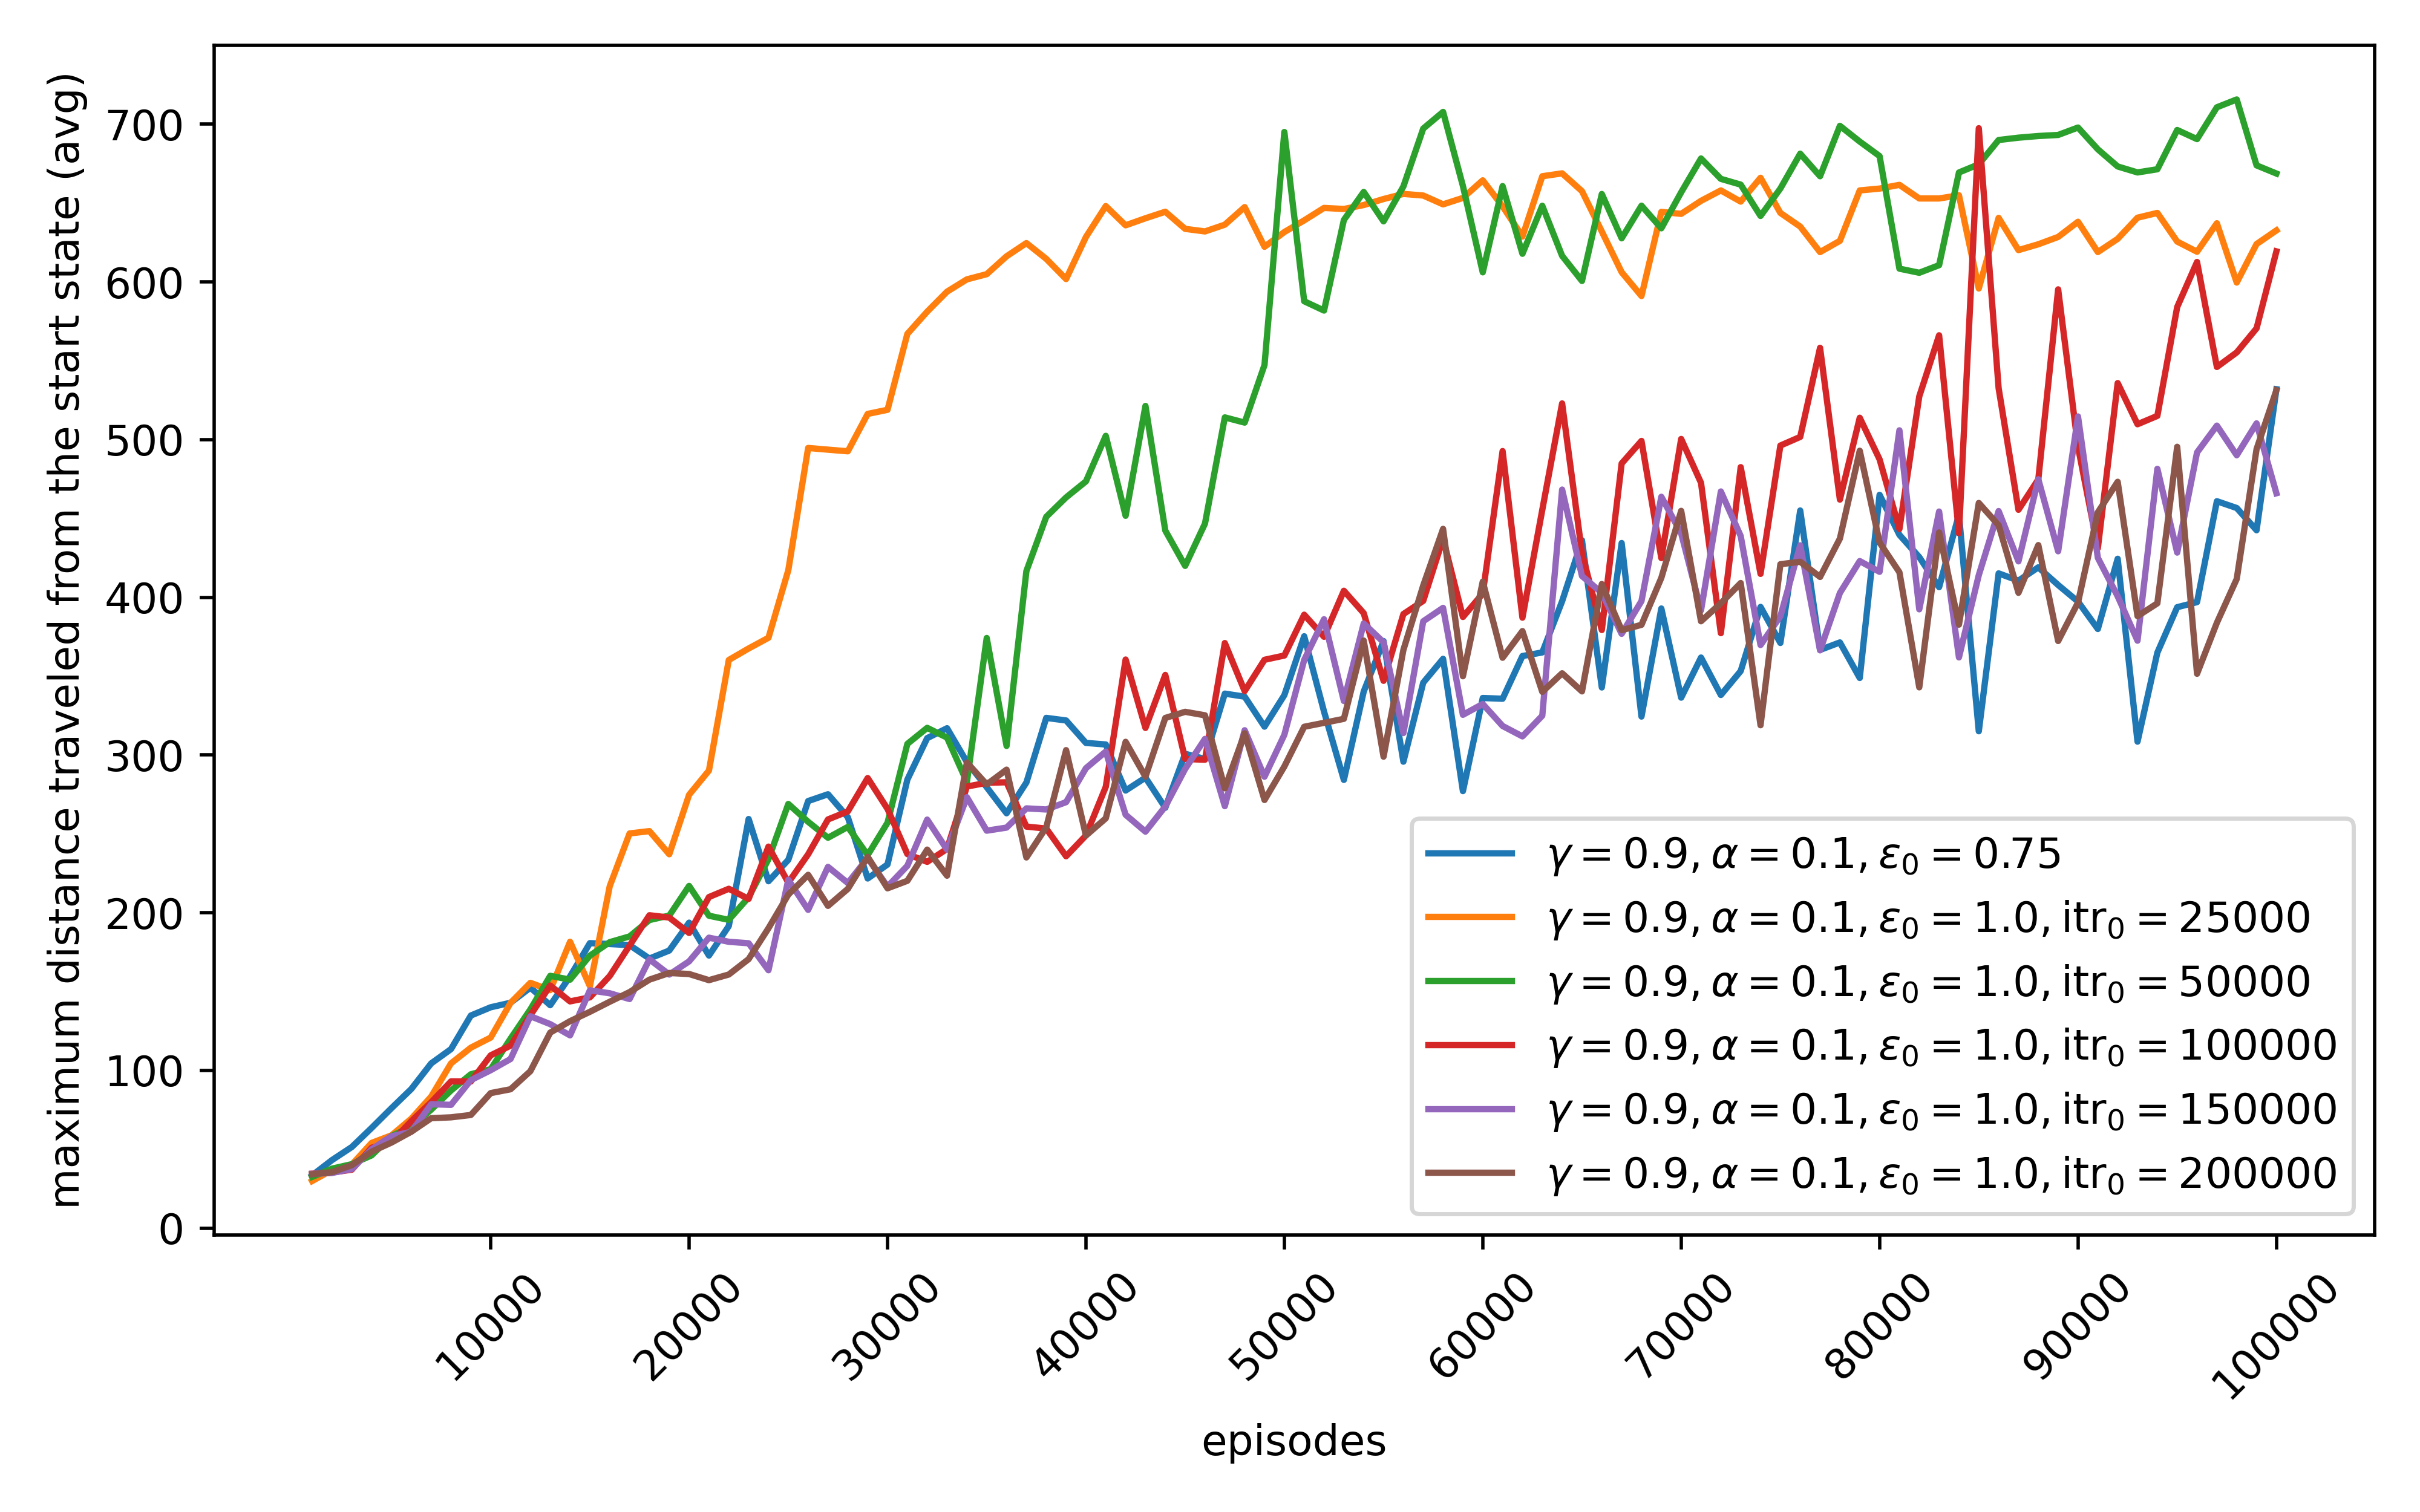
\includegraphics[width=\linewidth]{plots/part1-d.linear-distances.png}
        \caption{Distance Traveled}
    \end{minipage}
    \vspace{1em}

    % Third Row - Tables
    \begin{minipage}{0.49\linewidth}
        \centering
        \begin{tabular}{lcc}
        \hline
        $\texttt{itr}_0$ & Discounted Return & Average Distance \\
        \hline
        $25,000$ & $1.097$ & $632.68$\\ 
        $50,000$ & $1.108$ & $668.74$\\
        $100,000$ & $1.116$ & $619.39$ \\
        $150,000$ & $1.086$ & $466.01$ \\
        $200,000$ & $1.091$ & $531.35$ \\
        \hline
        \end{tabular}
        \caption{Linear Scheduling $\epsilon$}
        \label{tab:part1-d-linear}
    \end{minipage}
    \hfill
    \begin{minipage}{0.49\linewidth}
        \centering
        \begin{tabular}{lcc}
            \hline
            $\texttt{itr}_{1/2}$ & Discounted Return & Average Distance \\
            \hline
            $25,000$ & $1.097$ &  $483.09$\\
            $50,000$ & $1.099$ &  $484.38$\\
            $100,000$ & $1.103$ &  $467.94$\\
            $200,000$ & $1.094$ & $391.59$ \\
            $400,000$ & $1.096$ &  $400.47$\\
            \hline
        \end{tabular}
        \caption{Exponential Scheduling $\epsilon$}
    \end{minipage}
    \label{fig:part1-d}
    \caption{\texttt{Tabular} $100,000$ iterations, $\gamma = 0.9, \alpha = 0.1, \epsilon_0 = 1.0$} 
\end{figure}
In Linear Scheduling, Average Distance and Discounted Reward) peak at $\texttt{itr}_\texttt{0}$ $50,000$ and $100,000$ respectively. Too fast $\epsilon$ decay leads to starvation and too slow decay does not give the model enough opportunity to lean the optimum policy, given the knowledge of rewards explored. 


\section{Changing Environment}
\subsection{Overtake Reward}

\begin{figure}[H]
    \centering
    \begin{minipage}{0.49\linewidth}
        \centering
        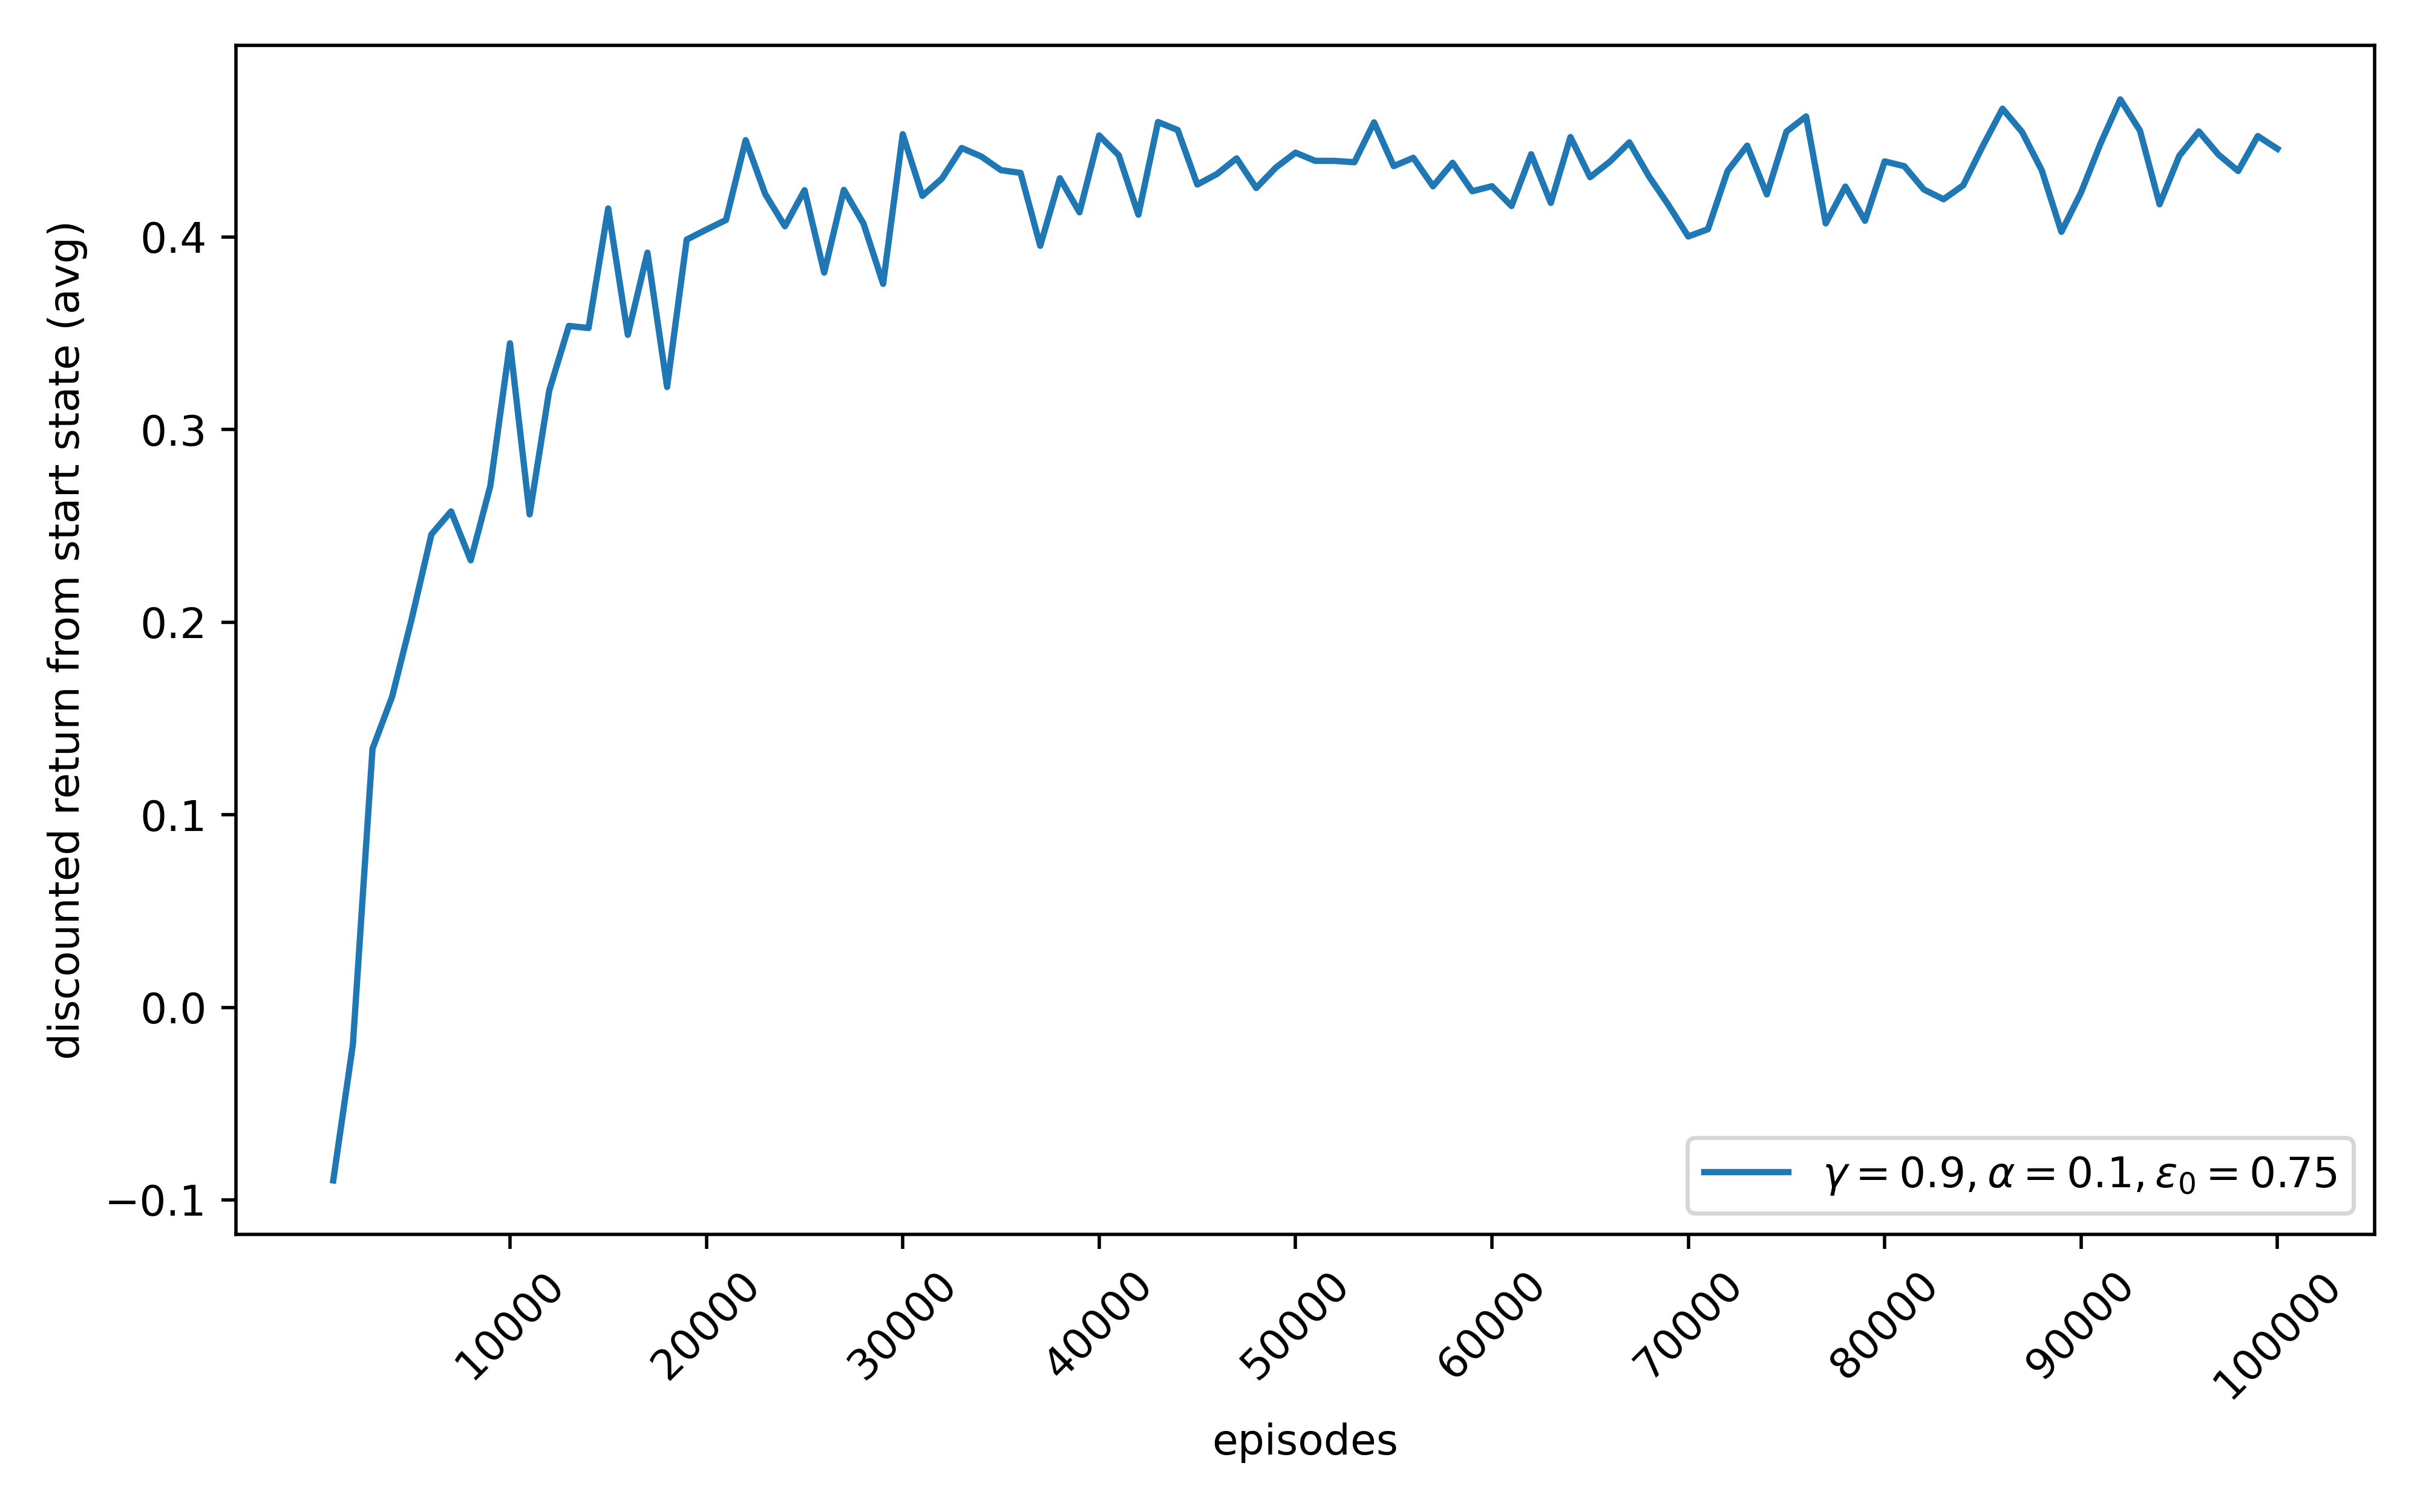
\includegraphics[width=\linewidth]{plots/part1-e.1-rewards.png}
        \caption{Discounted Return}
        
    \end{minipage}
    \hfill
    \begin{minipage}{0.49\linewidth}
        \centering
        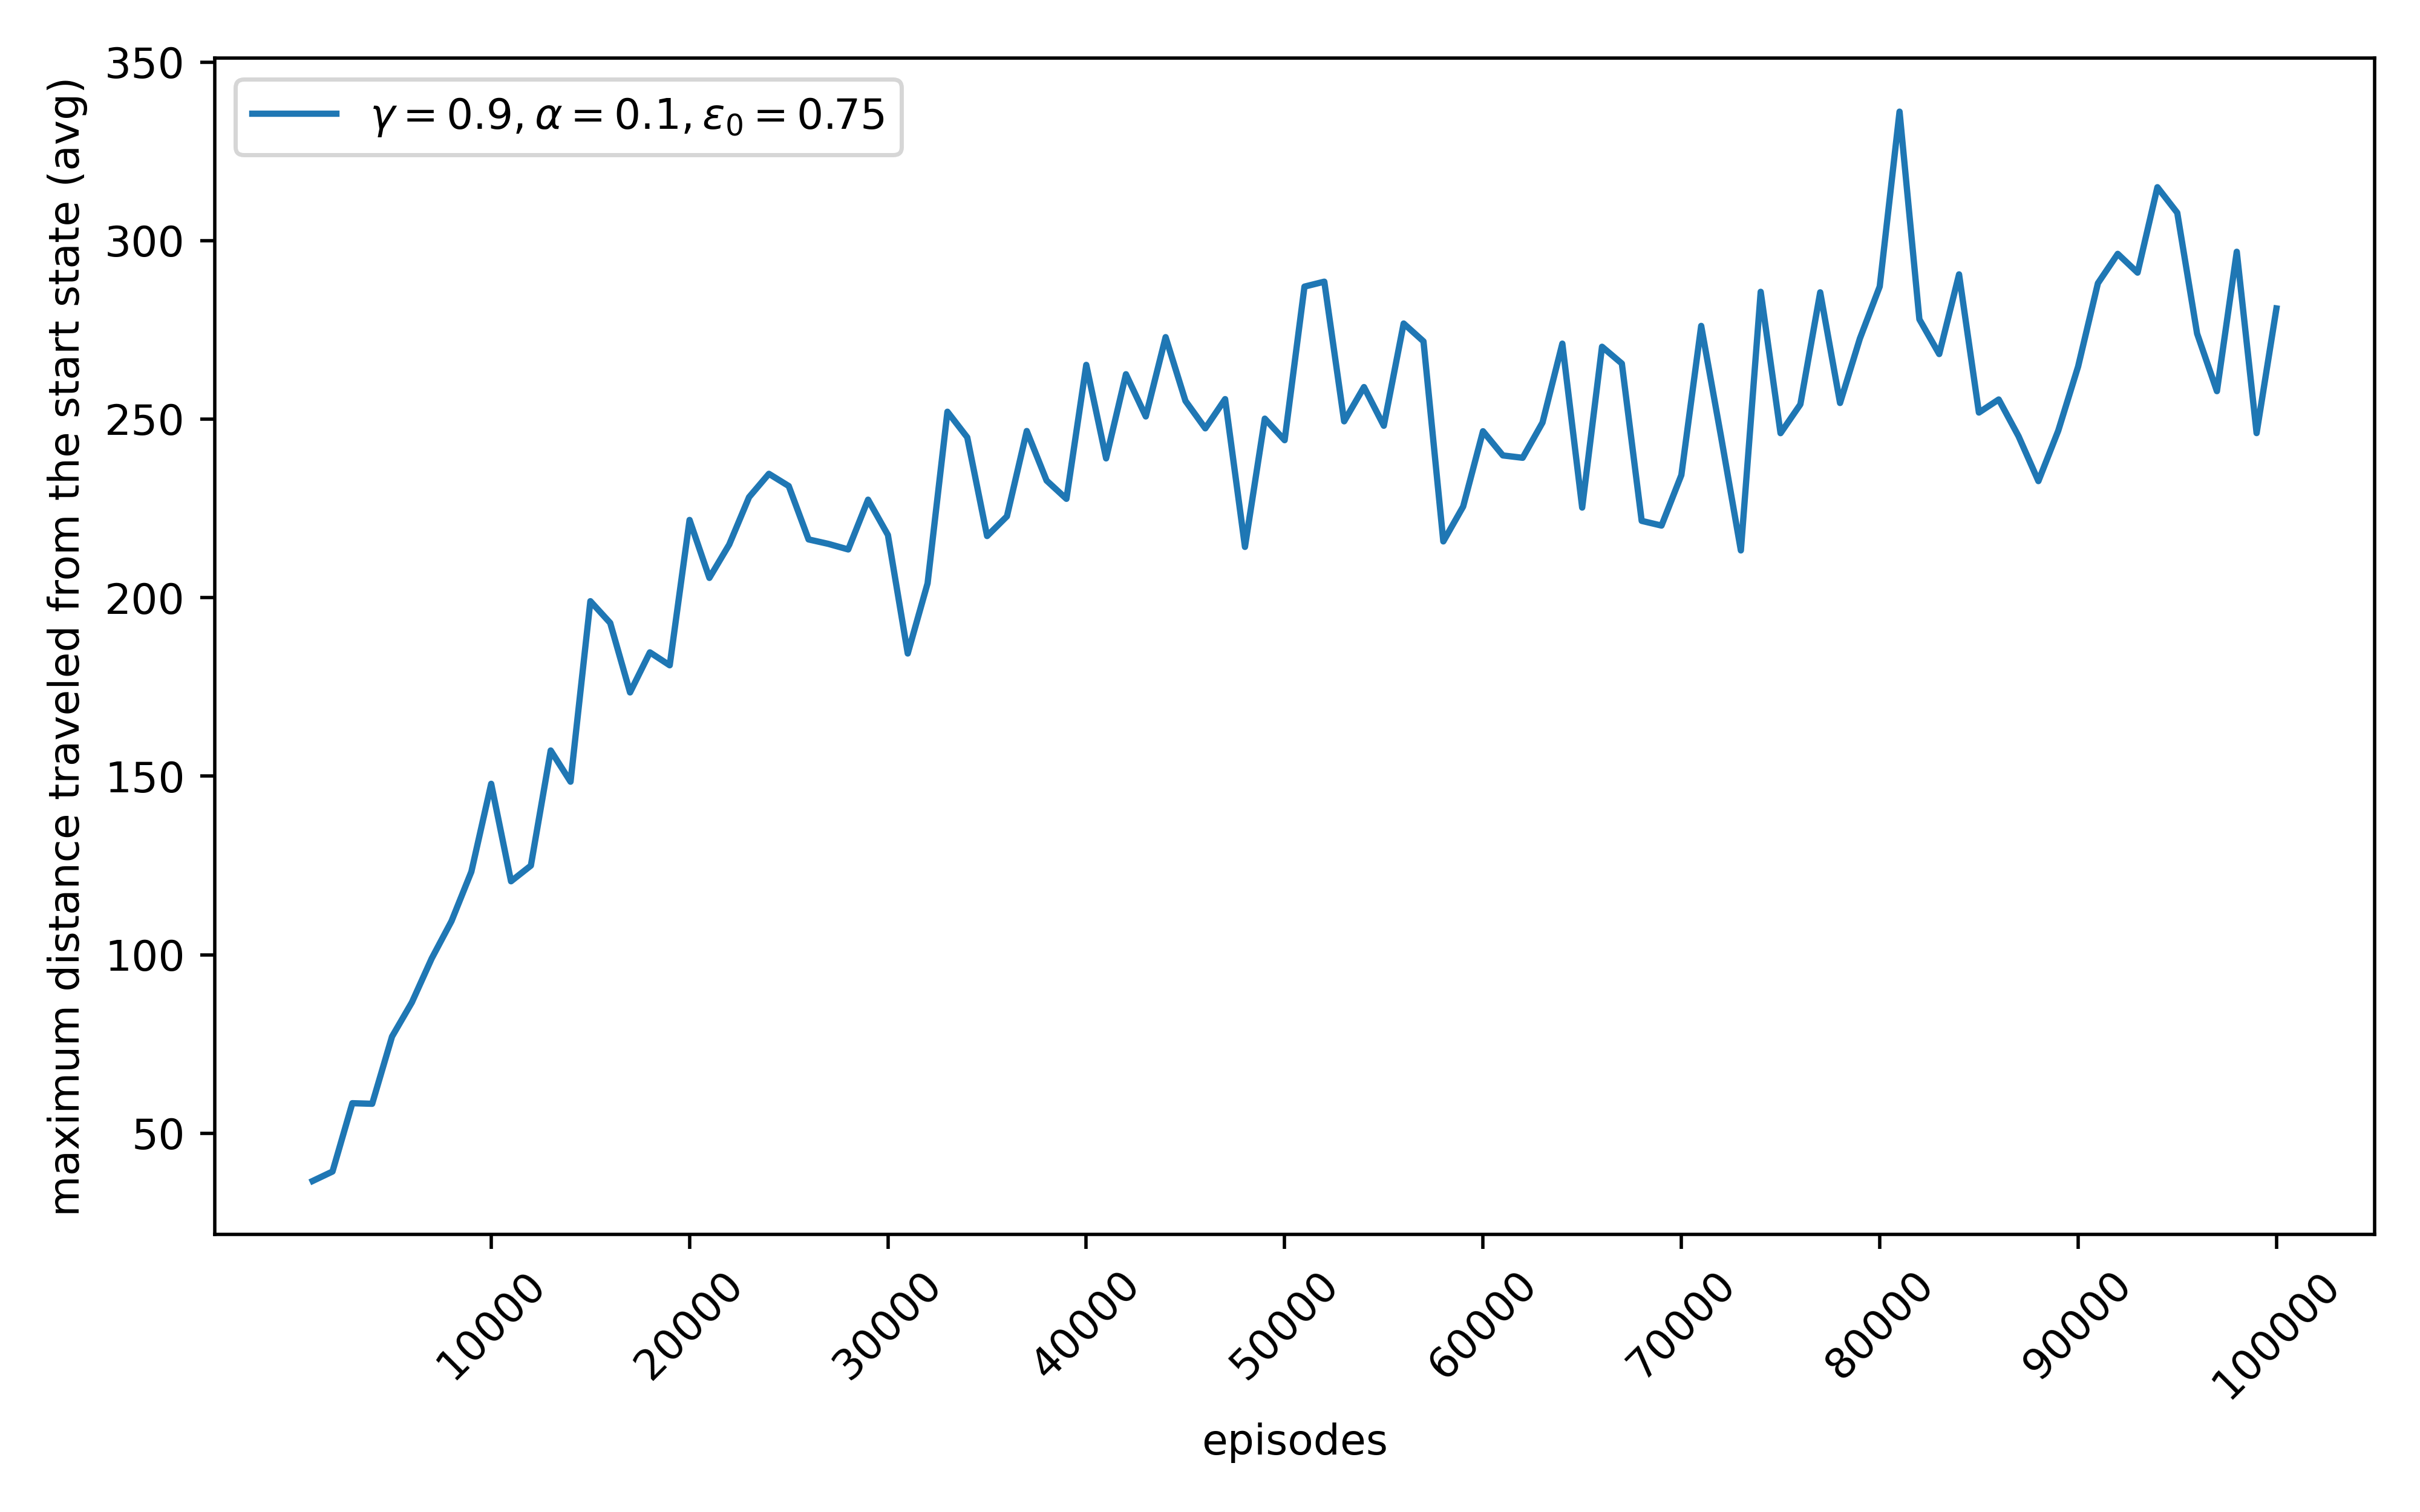
\includegraphics[width=\linewidth]{plots/part1-e.1-distances.png}
        \caption{Distance Traveled}
    \end{minipage}

    \vspace{1em}
    \begin{minipage}{\linewidth}
        \centering
        \begin{tabular}{lccc}
            \hline
            Episodes & Discounted Return & Average Distance \\
            \hline
            $98,000$ & $0.43$ & $296.87$ \\
            $99,000$ & $0.45$ & $246.07$ \\
            $100,000$ & $0.45$ & $280.99$ \\
            \hline
        \end{tabular}
        \caption{\texttt{Tabular} $\gamma = 0.9, \alpha = 0.1, \epsilon = 0.75$. Reward: \texttt{overtakes}.}
    \end{minipage}
     \label{fig:part1-e2}
\end{figure}

\begin{enumerate}
    \item From the \texttt{gifs} we observed that the agent drives faster (trying to overtake the other cars). This is in contrast to the case then reward is total distance traveled, where the agent tries to move in lanes that are empty and also reduces it's speed often in order to \textbf{remain far} from other car, to reduce chances of collisions with other cars.
\item Lane Visualization: See \autoref{fig:part1-e.1-lane-visualization}. We didn't see any clear difference from the total distance reward case. The agent prefers lanes where obstacles are farther away.
\item Speed Visualization:  See \autoref{fig:part1-e.1-speed-visualization}. The agent has a clear preference here for higher speeds, even when it is close to other cars, the agent doesn't assign higher value to slowing down, unlike when reward is total distance. 
\end{enumerate}

\begin{figure}[H]
    \centering
    \begin{minipage}{0.48\textwidth}
        \centering
        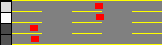
\includegraphics[width=\linewidth]{plots/part1-e.1-lane_visualization_01_step_0420.png}
    \end{minipage}
    \hfill
    \begin{minipage}{0.48\textwidth}
        \centering
        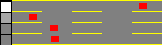
\includegraphics[width=\linewidth]{plots/part1-e.1-lane_visualization_00_step_1000.png}
    \end{minipage}
    \caption{Lane Visualization for Tabular Q-agent with \texttt{overtakes} reward}
    \label{fig:part1-e.1-lane-visualization}
\end{figure}

\begin{figure}[H]
    \centering
    \begin{minipage}{0.48\textwidth}
        \centering
        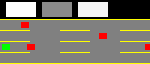
\includegraphics[width=\linewidth]{plots/part1-e.1-speed_visualization_02_step_0020.png}
    \end{minipage}
    \hfill
    \begin{minipage}{0.48\textwidth}
        \centering
        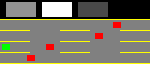
\includegraphics[width=\linewidth]{plots/part1-e.1-speed_visualization_00_step_0920.png}
    \end{minipage}
    \caption{Speed Visualization for Tabular Q-agent with \texttt{overtakes} reward}
    \label{fig:part1-e.1-speed-visualization}
\end{figure}




\subsection{Distance levels: $3$}

\begin{figure}[H]
    \centering
    \begin{minipage}{0.49\linewidth}
        \centering
        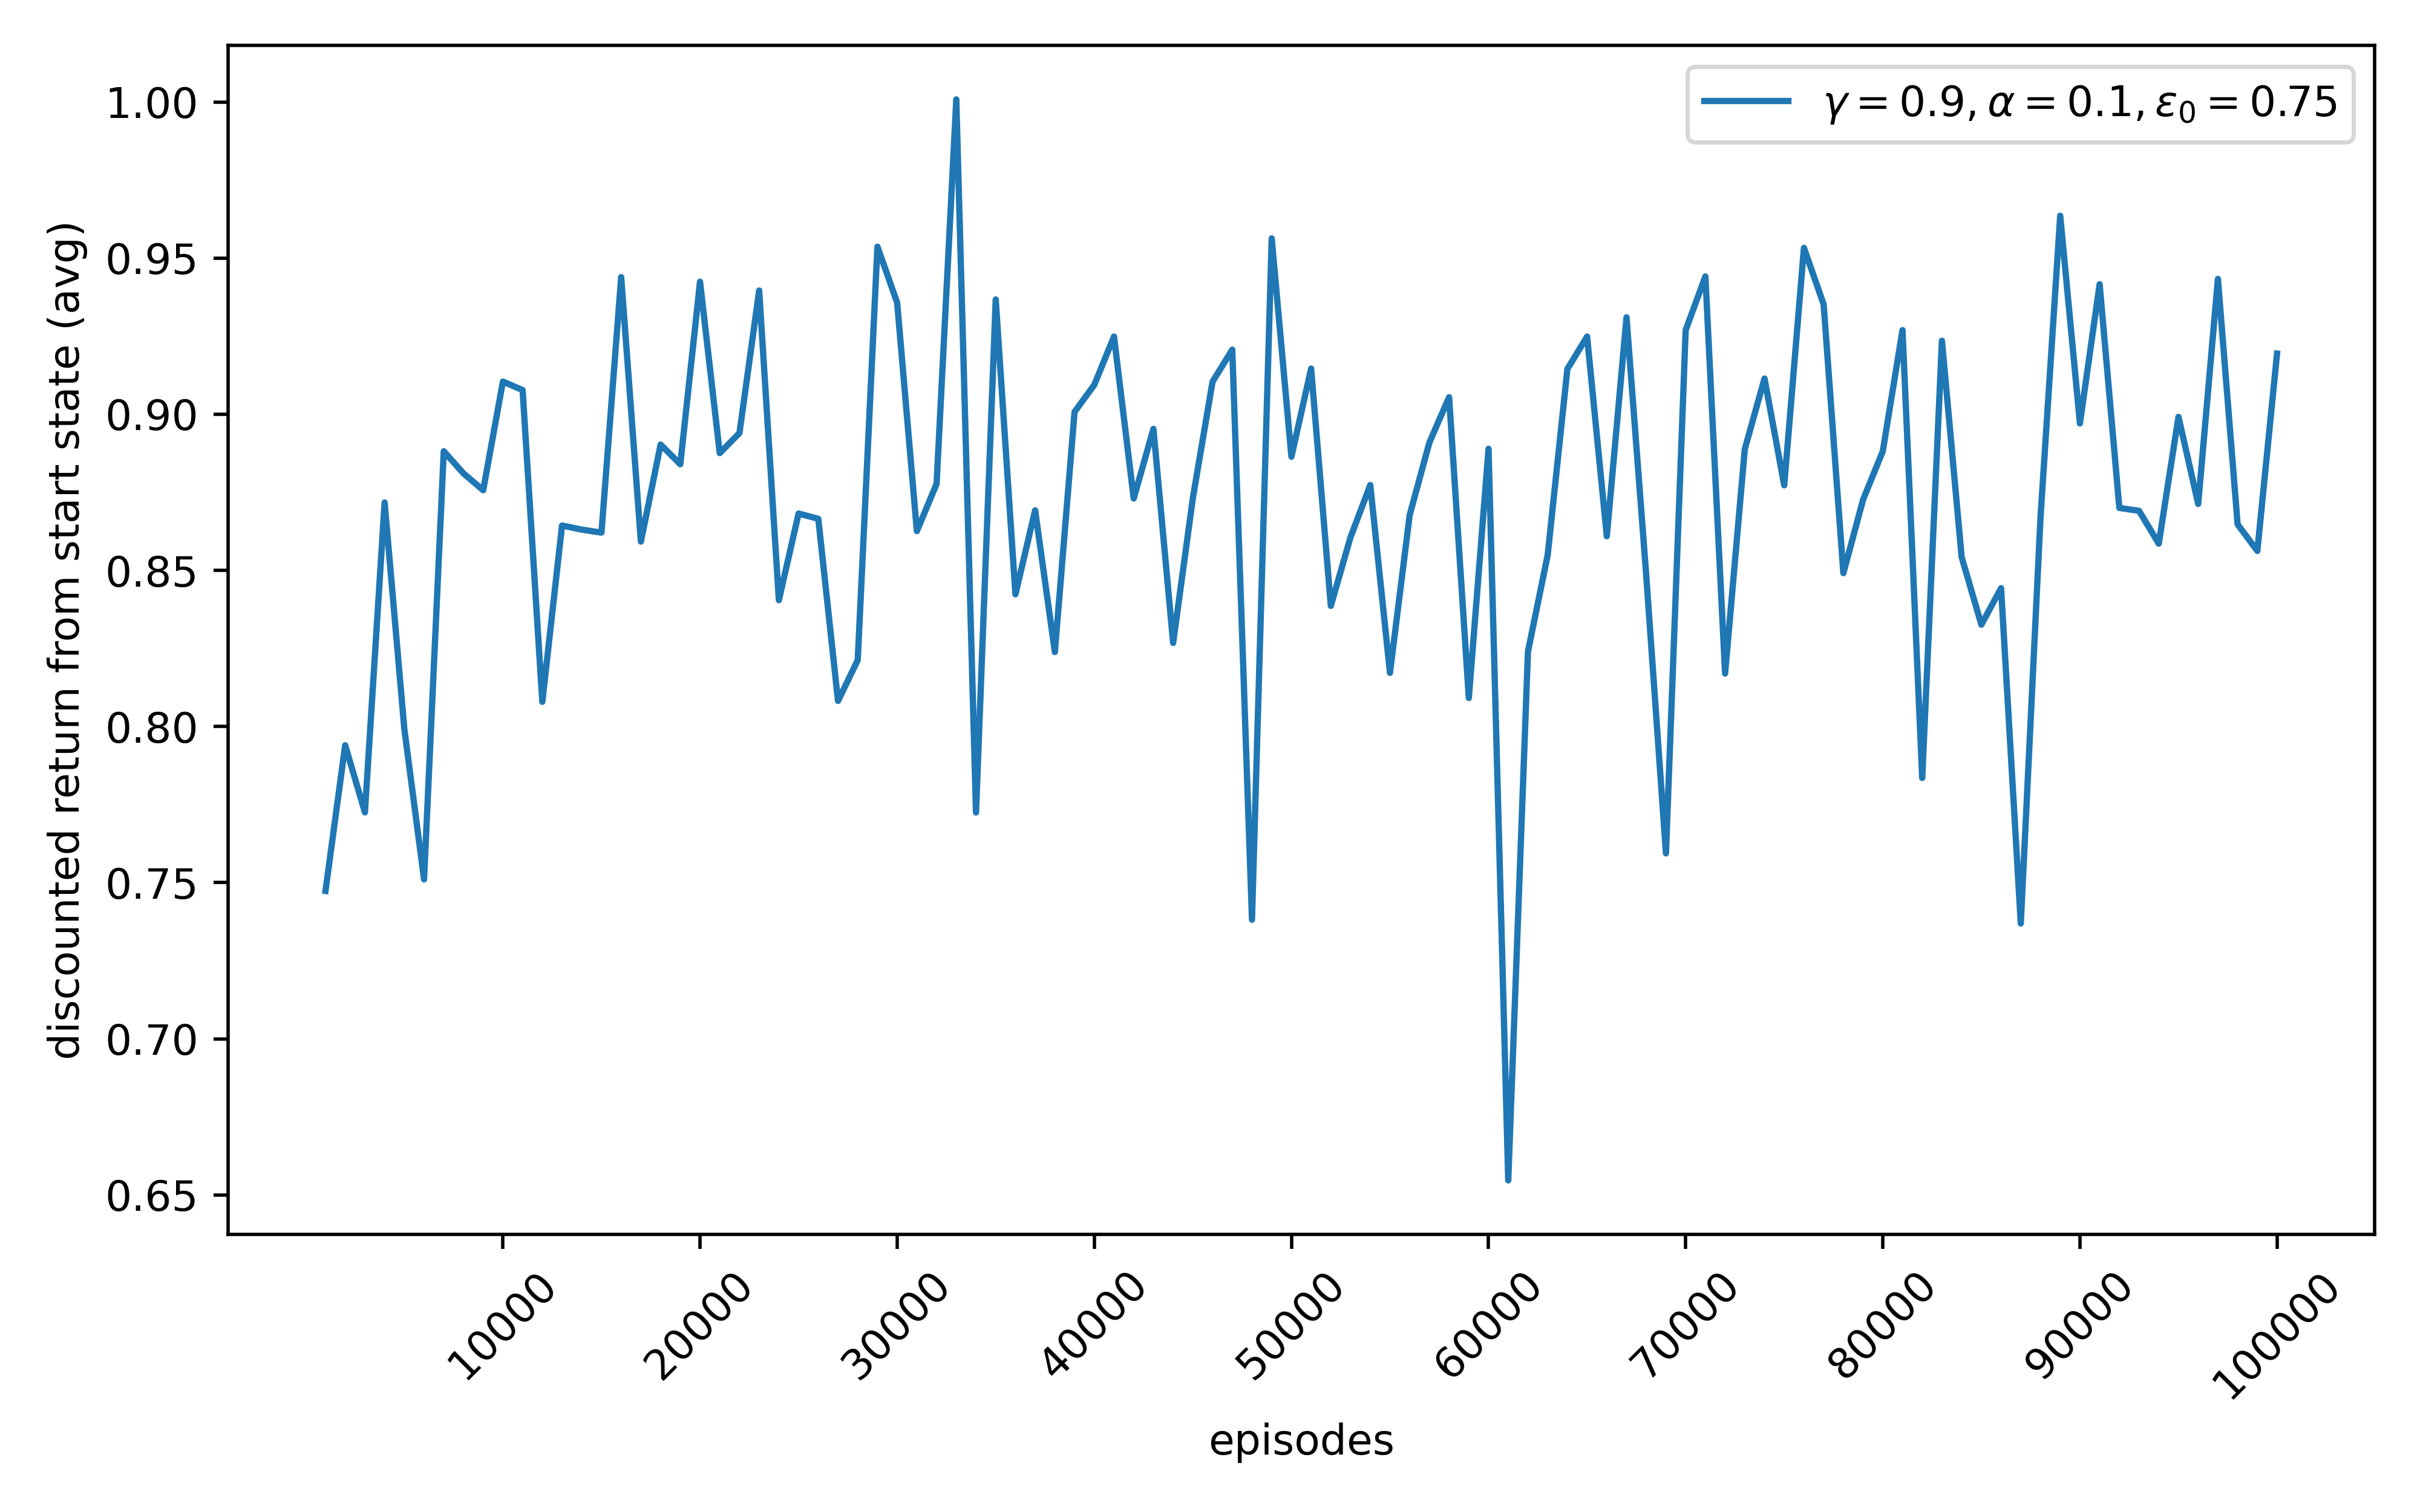
\includegraphics[width=\linewidth]{plots/part1-e.2-rewards.png}
        \caption{Discounted Return}
        
    \end{minipage}
    \hfill
    \begin{minipage}{0.49\linewidth}
        \centering
        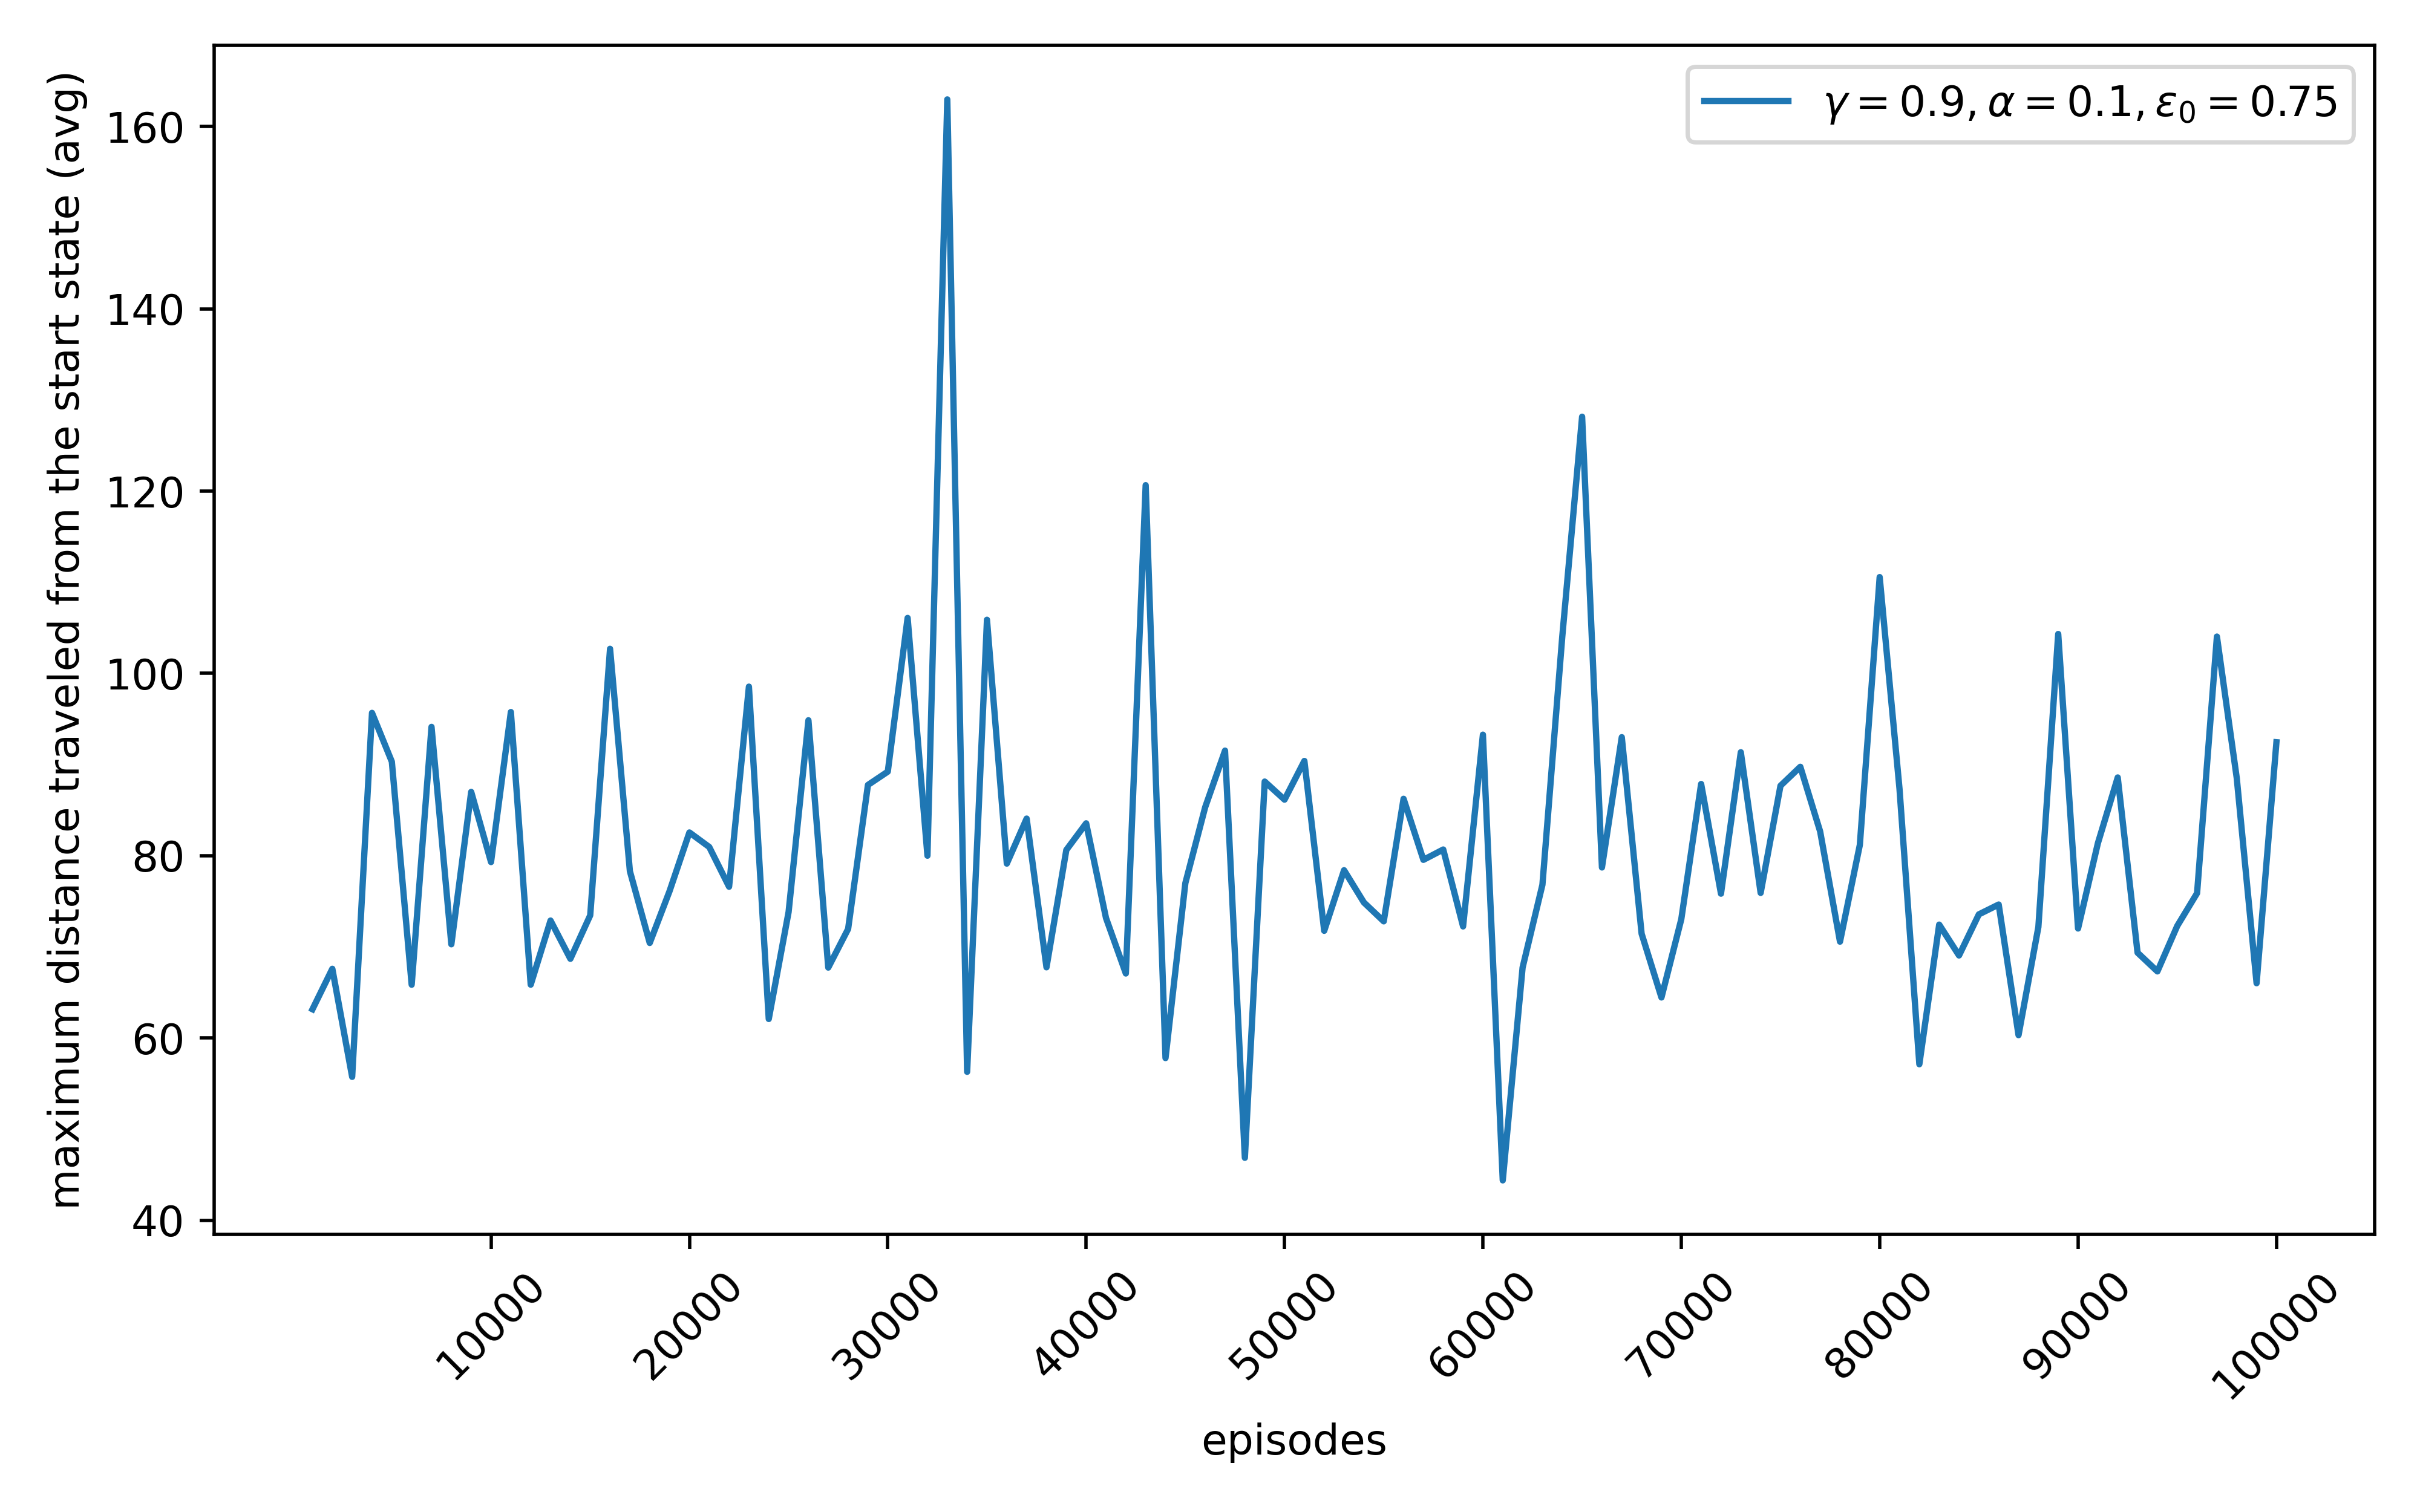
\includegraphics[width=\linewidth]{plots/part1-e.2-distances.png}
        \caption{Distance Traveled}
    \end{minipage}

    \vspace{1em}
    \begin{minipage}{\linewidth}
        \centering
        \begin{tabular}{lccc}
            \hline
            Episodes & Discounted Return & Average Distance \\
            \hline
            $98,000$ & $0.86$ & $88.52$ \\
            $99,000$ & $0.86$ & $66.02$ \\
            $100,000$ & $0.92$ & $92.46$ \\
            \hline
        \end{tabular}
        \caption{\texttt{Tabular} $\gamma = 0.9, \alpha = 0.1, \epsilon = 0.75$ and $3$ discrete levels of distance.}
    \end{minipage}
     \label{fig:part1-e2}
\end{figure}
\begin{enumerate}
\item We see that the total distance traveled is much less compared o the case of $5$ discrete levels. In the \texttt{gifs} we see that the agent starts "acting" (switching lanes) even when it is much far from the cars (compared to the $5$ levels case).

\item Lane Visualization: See \autoref{fig:part1-e.2-lane-visualization}. The agent is not able to differentiate well due to smaller level of discretization.
\item Speed Visualization:  See \autoref{fig:part1-e.2-speed-visualization}. Compared to \autoref{fig:part1-a-speed-visualization}, the difference is assigned value is lower for the similar settings. The obstacle has to come really close to the agent for it to notice.
\end{enumerate}

\begin{figure}[H]
    \centering
    \begin{minipage}{0.48\textwidth}
        \centering
        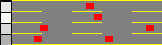
\includegraphics[width=\linewidth]{plots/part1-e.2-lane_visualization_00_step_0140.png}
    \end{minipage}
    \hfill
    \begin{minipage}{0.48\textwidth}
        \centering
        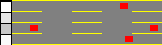
\includegraphics[width=\linewidth]{plots/part1-e.2-lane_visualization_00_step_0240.png}
    \end{minipage}
    \caption{Lane Visualization for Tabular Q-agent with $3$ levels of distance discretization}
    \label{fig:part1-e.2-lane-visualization}
\end{figure}

\begin{figure}[H]
    \centering
    \begin{minipage}{0.48\textwidth}
        \centering
        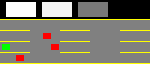
\includegraphics[width=\linewidth]{plots/part1-e.2-speed_visualization_00_step_0120.png}
    \end{minipage}
    \hfill
    \begin{minipage}{0.48\textwidth}
        \centering
        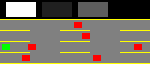
\includegraphics[width=\linewidth]{plots/part1-e.2-speed_visualization_00_step_0140.png}
    \end{minipage}
    \caption{Speed Visualization for Tabular Q-agent with $3$ levels of distance discretization}
    \label{fig:part1-e.2-speed-visualization}
\end{figure}
